\documentclass[final]{york-thesis}

\usepackage[utf8]{inputenc}
\usepackage[T1]{fontenc}
\usepackage{lmodern}
\usepackage[english]{babel}
\usepackage{array}
\usepackage{booktabs}
\usepackage{graphicx}
\usepackage{subcaption}
\usepackage{multirow}
\usepackage{enumitem}
\usepackage[bottom]{footmisc}
\usepackage{scalerel}
% \usepackage{afterpage}

\usepackage[width=.9\textwidth]{caption}
\setlength{\textfloatsep}{26pt plus 2.0pt minus 4.0pt}

% Copied from http://www.khirevich.com/latex/microtype/
%\usepackage[activate={true,nocompatibility},
%            final,tracking=true,kerning=true,
%            spacing=true,factor=1100,stretch=10,shrink=10]{microtype}
% activate={true,nocompatibility} - activate protrusion and expansion
% final - enable microtype; use "draft" to disable
% tracking=true, kerning=true, spacing=true - activate these techniques
% factor=1100 - add 10% to the protrusion amount (default is 1000)
% stretch=10, shrink=10 - reduce stretchability/shrinkability (default is 20/20)
%\microtypecontext{spacing=nonfrench}

%\usepackage{algpseudocode}
%\algrenewcommand{\algorithmicforall}{\textbf{for each}}
%\def\ForEach{\ForAll}

\usepackage{amsfonts}
\usepackage{amsmath}
\DeclareMathOperator*{\argmax}{argmax}

\usepackage[hyphens]{url}
\usepackage{relsize}
\renewcommand*{\UrlFont}{\ttfamily\relscale{0.93}}

\usepackage{tikz}
\usetikzlibrary{
  matrix,
  positioning,
  decorations.pathreplacing,
  decorations.markings,
  arrows.meta
}

\usepackage{fancyhdr}
\lhead{}\rhead{}
\lfoot{}\cfoot{\thepage}\rfoot{}
\renewcommand{\headrulewidth}{0pt}
\renewcommand{\footrulewidth}{0pt}

\usepackage[ocgcolorlinks,backref=page]{hyperref}
\hypersetup{
  linktocpage,
  colorlinks=true,
  linkcolor=blue,
  citecolor=blue,
  filecolor=blue,
  urlcolor=blue
}
% Bibliography with page numbers
% http://tex.stackexchange.com/a/15977
%\renewcommand*{\backref}[1]{}
%\renewcommand*{\backrefalt}[4]{%
%    \ifcase #1 (Not cited.)%
%    \or        (Cited on page~#2.)%
%    \else      (Cited on pages~#2.)%
%    \fi}
% http://tex.stackexchange.com/q/110679
%\backrefsetup{disable}

\usepackage[numbers,sort&compress]{natbib}
\usepackage{hypernat}

\title{Strong Field Interactions with Atoms and Molecules}
\author{Susana Arias Laso}
\date{\today}
\hypersetup{
  pdftitle={Strong Field Interactions with Atoms and Molecules},
  pdfauthor={Susana Arias Laso}
}

\setboolean{masters}{false}
\degreename{Doctor}
\masterof{Arts}
\department{Physics and Astronomy}

\setboolean{hasfigures}{true}
\setboolean{hastables}{true}

\abstractfile{abstract.tex}
%\acknowledgementsfile{acknowledgements.tex}
\abbreviationsfile{abbreviations.tex}

\begin{document}

%\microtypesetup{protrusion=false}
\spacing{1.48}  % Make the Table of Contents fit in two pages.
\makefrontmatter
\spacing{1.5}
%\microtypesetup{protrusion=true}

\backrefsetup{enable}
\chapter{Introduction}
\label{cha:introduction}

ref~\cite{sarias_2016}

%%% Local Variables:
%%% mode: latex
%%% TeX-master: "thesis"
%%% End:


\chapter{Electronic Structure of H$_{2}$O}
\label{cha:scf_h2o}

% read
% references -> Rootham-Hartree-Fock -> RoothaanRevModPhys(1951).pdf
% books -> Levine -> ch.15, ch.11

% mention the Ellison and Shull calculations on H2O that are reference

% initial calculations of the water molecule carried out by means of a
% multicentre HF evaluation of Slater-type orbitals

% approach implemented by Moccia, described in JChemPhys40_2164

This chapter presents a brief compilation of the principles of the
Hartree-Fock (\textsc{hf}) formulation implemented in problems of
molecular quantum mechanics. Section~\ref{ch:var_hf} summarizes the
principles in the Roothaan formulation of the Hartree-Fock formalism,
in which the Hartree-Fock orbitals are expressed as linear
combinations of suitable analytical functions~\cite{Roothaan_HF}. For
molecules, the calculation of electronic wavefunctions is more
intricate than that for atoms since it is preferable to use basis
functions centred about the several
nuclei~\cite{Pitzer_1968,Pitzer_1970}. This implies the difficult task
of evaluating multicentre integrals. Sec.~\ref{ch:scf_sto} describes a
different approach that consists of using a set of basis functions all
referred to one common origin and has reported satisfactory results in
calculations of self-consistent field molecular orbitals of
AH$_{n}$-type molecules~\cite{Moccia_JCP_2164, Moccia_1964}.


\section{Variational Hartree-Fock Method}
\label{ch:var_hf}
% HF self-consistent field method to determine molecular orbitals

% define starting point to determine the fock equations

% define AP (antisymmetrized product)

% state fosk's equations

% describe Roothaan's SCF method for a closed-shell ground state
% (linear combination of atomic orbitals)

The starting point in the Hartree-Fock self-consistent field
(\textsc{scf}) method is the antisymmetrized product (\textsc{ap}) of
$N$ one-electron wave functions, called molecular spinorbitals, which
contain space and spin coordinates of the
electrons~\cite{Roothaan_HF},
% insert equation of the AP here
%
\begin{eqnarray}
  \begin{split}
    \Phi & = & \sqrt{N!}\psi_{1}^{[1} \psi_{2}^{2} \cdots \psi_{N}^{N} =
    (N!)^{-1/2}
    \begin{vmatrix}
      \psi_{1}^{1} & \psi_{2}^{1} & \cdots & \psi_{N}^{1} \\
      \psi_{1}^{2} & \psi_{2}^{2} & \cdots & \psi_{N}^{2} \\
      \cdots & \cdots & \cdots & \cdots \\
      \psi_{1}^{N} & \psi_{2}^{N} & \cdots & \psi_{N}^{N}
    \end{vmatrix}
  \end{split},
  \label{eq:AP}
\end{eqnarray}
%
where the superscripts $[1\ 2 \cdots N]$ indicate that one must
consider all the permutations of the sequence $1\ 2 \cdots N$ such
that the Pauli principle is satisfied, that is, each \textsc{mo}
$\varphi_{i}$ may occur not more than twice (corresponding to opposite
spin signs) in the product wave function.





\section{Self-Consistent Field Slater Orbitals}
\label{ch:scf_sto}

% Slater orbitals in Moccia's calculations following Roothaan procedure



%%% Local Variables:
%%% mode: latex
%%% TeX-master: "thesis"
%%% End:

\chapter{H$_{2}$O in an external electric dc field}
\label{ch:dc_h2o}

% H2O in strong dc fields
% effective potential
% outline of the chapter

The stark resonance parameters, which characterize the shift of the
molecular energy levels under an external dc field, are fundamental in
the study of the strong dc field ionization of molecular orbitals
(\textsc{mo}s). In the case of the water molecule, the multicentre
nature of the combined Coulomb interactions and, consequently, the
additional degrees of freedom, make the strong dc field ionization of
H$_{2}$O an attractive and challenging problem from the point of view
of a theoretical description as well as experimentally. Complex
variable techniques, such as an exterior complex
scaling~\cite{Simon_1979,ecsScrinzi} and complex-absorbing
potentials~\cite{RissMeyer_1993,Krause_2014}, have been implemented in
order to address the problem of molecular static-field ionization and
compute the induced Stark resonances.

The dc Stark problem for the H$_{2}$O valence orbitals is addressed in
this chapter by the implementation of a modified exterior complex
scaling approach that allows to study the ionization of the molecular
orbitals of H$_{2}$O under a strong dc field. The construction of an
effective potential, which reflects the indivual properties of the
orbitals, is crucial in this analysis. In Sec.~\ref{ch:h2o_structure},
we formulate the problem with emphasis on the representation of the
molecular orbitals. The exterior complex scaling formalism is
introduced in Secs.~\ref{ch:1b1_1b2} and~\ref{ch:3a1} as a crucial
step in finding a numerical solution to a spherically symmetric
problem, in the case of the $1b_{1}$ and $1b_{2}$ orbitals, and the
problem of a non-central effective potential, in the case of the
$3a_{1}$ orbital. The Stark resonance parameters are then presented in
Sec.~\ref{ch:stark_params}, in which the symmetry properties of the
orbitals are considered independently. The analysis presented in this
chapter compiles that of~\cite{sarias_2016,sarias_2017}.


\section{Non-Hermitian quantum mechanics}
\label{ch:nonH_qm}
% introduction of the basic principles of this formulation of QM
% introduce complex-variable methods used later on: ECS and CAP

The study of resonance phenomena, such as atomic and molecular
strong-field ionization events, has been successfully approached
within the framework of non-Hermitian quantum
mechanics~(\textsc{nhqm})~\cite{Moiseyev_NHQM}. This alternative
formulation to the standard formalism of quantum mechanics allows for
a time-independent interpretation of strong-field ionization processes
and quantitative modelling of the associated ionization rates. This is
possible by means of implementing analytic continuation methods on the
Hamiltonian, from which the resonance is obtained as a solution with
complex eigenvalues of the form
%
\begin{eqnarray}
  E = E_{R} + i E_{I} = E_{R} - i \Gamma/2,
  \label{eq:complex_eigenE}
\end{eqnarray}
%
in which the ionization rate, $\Gamma$, induced by the external field
$F_{0}$ is associated to the lifetime of the decaying state $\tau$ via
$\Gamma\tau = 1$, while the real part $E_{R}$ represents the Stark
shift under the external field.

Several numerical techniques have been introduced within the framework
of \textsc{nhqm} that implement a complex-scaled Hamiltonian in
studies of atomic and molecular Stark resonances. It is the scope of
this work to focus on two of these methods to study the response of
the H$_{2}$O highest-energy orbitals to an external dc-field, the
concept of a complex absorbing potential~(\textsc{cap}) introduced as
a perturbation to the molecular Hamiltonian and exterior complex
scaling~(\textsc{esc}).

% add artificial potential introduced to absorb outgoing wave

% relevant parameters in a CAP (equation for the CAP used in the
% partial wave calculations)

% approach to obtain the resonances (to remove the perturbation
% introduced by the CAP)

A \textsc{cap} is introduced as an imaginary potential which allows an
analytical continuation of the Hamiltonian to the complex plane. This
artificial perturbation of the system acts as an effective potential
that suppresses the diverging tail of the resonance wave function in
the vicinity of the edges of a numerical grid. As a result, the
solutions of the modified non-Hermitian Hamiltonian behave as
square-integrable eigenstates within the original boundary conditions.

In general terms, the application of a \textsc{cap} begins with the
addition of an artificial local potential of the form $-i \eta W(r)$
to the Hamiltonian of the system, where the parameter $\eta$ indicates
the strength of the \textsc{cap}. The function $W(r)$, which
determines the onset of the \textsc{cap}, has been most commonly
defined as a quadratic potential centred at some radius
$r_{\mathrm{c}}$. The \textsc{cap} approach requires calculating sets
of complex eigenvalues along complex trajectories, $E(\eta)$,
determined by the \textsc{cap} strength in order to find an optimal
finite value of $\eta$ such that it makes the resonance stable, with
the ultimate goal of removing the perturbation by the \textsc{cap}.

Strategies used to obtain the optimal value of $\eta$ include the
Pad\'{e}-approximation-extrapolation
procedure~\cite{Moiseyev_Pade_2005}, and Riss-Meyer iterative
method~\cite{RissMeyer_1993}. Such correction schemes applied to
complex scaling methods have proven to yield accurate values for the
Stark resonance parameters for diatomic molecules, such as the
hydrogen molecular ion, in a static electric field with a
\textsc{cap}~\cite{Tsog_2013}.
% add references cited in the partial wave write-up and Moiseyev book on NHQM
  




% JAGAU REVIEW ON CS
% In the limit η → 0, the spectrum becomes continuous, and for each
% resonance there exists an eigenvalue of Hη that converges to the
% exact resonance position and width provided that W goes to infinity
% for r → ∞, is piecewise continuous, and satisfies a few more general
% requirements (35). That is, an infinitesimally weak CAP (η → 0) is
% sufficient to stabilize the resonance without perturbing it.


% The commonly used strategy for finding an optimal value of η is to
% compute trajectories, E(η), and then determine ηopt through (35, 46)
% min|η dE/dη|. The rationale for this criterion is that it minimizes
% the first-order term in a Taylor expansion of the energy in η (35),
% but unfortunately, the resonance position and width computed using
% this criterion are very sensitive to the CAP onset (46, 60, 100).


\section{Molecular orbital representation of H$_{2}$O}
\label{ch:h2o_structure}
% Formulation of the Problem

The starting point for this study is the Hartree-Fock (\textsc{hf})
calculation of the H$_{2}$O molecular states using a single-center
Slater orbital
basis~\cite{Moccia_1964,Moccia_JCP_2164,Moccia_JCP_2176}, applied to
collision studies~\cite{Montanari_2013} and compared to experimental
electron spectroscopy~\cite{Hafied_2007}. Other elaborate descriptions
of the molecular structure of H$_{2}$O formulated within the
independent-electron approximation by the self-consistent field
(\textsc{scf}), or variational Hartree-Fock method with multicentre
Slater orbitals, in which the pioneering work of Ellison and
Shull~\cite{EllisonShullh2o_1955} is revised, are reference for
describing the electronic structure of diatomic molecules by means of
an expansion of Slater
orbitals~\cite{Pitzer_1968,Pitzer_1970}. However, the direct
application of these multicentre orbitals for strong-field studies
implies significant computational and methodological challenges.

The present work is intended to study the valence molecular orbitals
of H$_{2}$O, $1b_{1}$, $1b_{2}$ and $3a_{1}$. The wavefunctions for
the $1b_{1}$ and $1b_{2}$ molecular orbitals, which correspond to the
$2p_{x}$ and $2p_{y}$ oxygen orbitals, are dominated by a single
angular mometum symmetry. The $3a_{1}$ \textsc{mo}, on the other hand,
consists mainly of the oxygen $2s$ and $2p_{z}$ and the hydrogen $1s$
atomic orbitals.

The general expression for the basis functions, introduced as a set of
single-center
wavefunctions~\cite{Moccia_1964,Moccia_JCP_2164,Moccia_JCP_2176}, is a
Slater-type orbital as defined in Eq.~(\ref{eq:f_STO}). The expansion
coefficients and nonlinear coeficients $\{\zeta_{i}\}$, determined by
the Roothaan's self-consistent-field
method~\cite{Moccia_1964,Roothaan_1951} introduced in
Sec.~\ref{ch:scf_sto}, are used to construct a reduced form of the
radial functions that describe all the molecular orbitals. More
specifically, we are interested in using a reduced \textsc{sto}
expansion to construct an effective pontential that describes the
response of the H$_{2}$O valence orbitals when applying an electric dc
field along the symmetry axis (i.e., the $z-$axis).

Based on their symmetry properties, independent descriptions of the
valence molecular orbitals of H$_{2}$O are constructed. The dominant
components of the $1b_{1}$ and $1b_{2}$ orbitals, namely the $np_{x}$
and $np_{y}$ parts, are used to derive spherically symmetric effective
orbital-dependent potentials~\cite{sarias_2016}. While a similar
procedure is implemented for the $3a_{1}$ orbital, i.e., retaining the
$np_{z}$ parts of the \textsc{mo}, the strong asymmetry introduced by
the two protons located in the $y-z$ plane leading to significant
admixtures of $s-$type Slater orbitals in the Moccia
\textsc{sto}s~\cite{Moccia_1964} would have been ignored with a
spherically symmetric potential. Hence, for the dc ionization problem
of the $3a_{1}$ \textsc{mo}, \textsc{sto}s of type $2s$ and $2p_{z}$
are incorporated in the analysis.


% representation of the orbitals, fig.1 in the papers (also fig.2 of
% the jphysb), with related comments

\section{$1b_{1}$ and $1b_{2}$ molecular orbitals}
\label{ch:1b1_1b2}

The Schr\"{o}dinger equation for the bound-state problem of a
molecular orbital within an effective potential $V_{\mathrm{eff}}(r)$
is expressed in shperical polar coordinates as
%
\begin{eqnarray}
  [ -\frac{1}{2} \frac{d^2}{dr^2} + \frac{\hat{L}^2}{2r^2} + V_{\rm{eff}}(r)] \psi
  & = & E\psi,
\label{eq:sch_noCS}
\end{eqnarray}
%
where $\hat{L}^{2}$ is the orbital quantum momentum operator. The
present study involves the construction of the effective
orbital-dependent potential, $V_{\mathrm{eff}}(r)$, extracted from the
single-centre Moccia wave functions~\cite{Moccia_1964}. This is
followed by the implementation of an exterior complex scaling
(\textsc{ecs})~\cite{Simon_1979} to determine the numerical solution
of the problem associated with a molecular orbital in the presence of
a strong electric dc field applied along the
$\hat{z}-$direction~\cite{sarias_2016}. A schematic representation of
the geometry of the system is shown in Figure~\ref{fig:h2o_1b1_1b2},
where the orientation of the $1b_{1}$ and $1b_{2}$ \textsc{mo}s is
indicated with respect to the plane where the protons are located. The
direction of the applied electric field along $\hat{z}$ is included as
well.

\begin{figure}
  \centering
  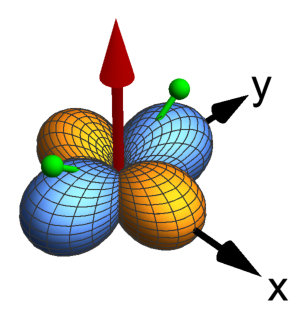
\includegraphics[width=0.25\textwidth]{figures/ch_H2O/1b1_1b2/orbitals.eps}
  \caption{Schematic display of the $1b_{1}\approx 2p_{x}$ (shown in
    yellow along the $x$ axis) and $1b_{2}\approx 2p_{y}$ (shown in
    blue along the $y$ axis) molecular orbitals. Also indicated (in
    green on the $y-z$ plane) is the orientation of the protons. The
    $z$ axis (in red) is the direction of the external electric field
    of strength $F_{0}$.}
  \label{fig:h2o_1b1_1b2}
\end{figure}


As a first step in solving Eq.~(\ref{eq:sch_noCS}) for the H$_{2}$O
molecular orbitals, we introduce the reduced single-centre Moccia
wavefunction,
%
\begin{eqnarray}
  \begin{split}
    \psi_{1b_{1},1b_{2}}(r) & = & \sum\limits_{i} c_{nlm} f_{nlm}(\zeta_{i}, r),
    \label{eq:sto_1b1_1b2}
  \end{split}
\end{eqnarray}
%
which approximates the molecular orbital by an eigenstate of a
spherically symmetric potential. The functions $f_{nlm}(\zeta_{i},r)$
represent the radial part of the Slater orbitals~(\ref{eq:sto}) with
$|m|=1$ for the magnetic quantum number, in which the \textsc{sto}
expansion is limited to $2p_{x}$ and $2p_{y}$ orbitals,
respectively. The set of expansion coefficients and non-linear
coefficients in~(\ref{eq:sto_1b1_1b2}), indicated in
Table~\ref{tab:1b11b2_coef}, represents a reduced selection of the
expansion parameters given by Moccia for the ground state of the water
molecule~\cite{Moccia_1964}.

\begin{table}[t]
 \centering
  \caption{\label{tab:1b11b2_coef} Expansion coefficients and
    nonlinear coefficients for the $1b_{1}$ and $1b_{2}$ molecular
    orbitals of H$_{2}$O. The parameters used in our reduced
    \textsc{sto} expansion are indicated as included.}
  \begin{tabular}{lrrrr}
    \toprule
    $(n,l, m)$ & & $\zeta_{i}$ & $c_{nlm}^{1b_{1}}$ & $c_{nlm}^{1b_{2}}$ \\
    \midrule
    $(2,1,1)$ & included & $1.510$ & $0.72081$ & --~~ \\
    $(2,1,1)$ & included & $2.440$ & $0.11532$ & --~~ \\
    $(2,1,1)$ & included & $3.920$ & $0.24859$ & --~~ \\
    $(3,2,1)$ & excluded & $1.600$ & $0.05473$ & --~~ \\
    $(3,2,1)$ & excluded & $2.400$ & $0.00403$ & --~~ \\
    $(4,3,1)$ & excluded & $1.950$ & $0.00935$ & --~~ \\
    $(4,3,3)$ & excluded & $1.950$ & $-0.02691$ & --~~ \\
    $(2,1,-1)$ & included & $1.510$ & --~~ & $0.88270$ \\
    $(2,1,-1)$ & included & $2.440$ & --~~ & $-0.07083$ \\
    $(2,1,-1)$ & included & $3.920$ & --~~ & $0.23189$ \\
    $(3,2,-1)$ & excluded & $1.600$ & --~~ & $0.25445$ \\
    $(3,2,-1)$ & excluded & $2.400$ & --~~ & $-0.01985$ \\
    $(4,3,-1)$ & excluded & $1.950$ & --~~ & $0.04526$ \\
    $(4,3,-3)$ & excluded & $1.950$ & --~~ & $-0.06381$ \\
    \bottomrule
  \end{tabular}
\end{table}

In order to determine the effective potential corresponding to each
molecular orbital, the wavefunction~(\ref{eq:sto_1b1_1b2}) is inserted
into the single-electron Schr\"{o}dinger equation~(\ref{eq:sch_noCS}),
which is then solved for $V_{\mathrm{eff}}^{(1)}(r)$. Afterwards, the
so-called Latter correction~\cite{LatterCor_1955,sarias_2016} is
applied to ensure that the effective potential converges
asymptotically to $-1/r$, as expected in a Coulomb potential:
%
\begin{eqnarray}
V_{\mathrm{eff}}(r) = \left\{
\begin{split}
V_{\mathrm{eff}}^{(1)}(r)\  & \mathrm{for} & r < r_{0} \\
-1/r\  & \mathrm{for} & r > r_{0}
\end{split}
\right.
,
\label{eq:coulomb_tail}
\end{eqnarray}
%
where the point $r_{0}$ is determined from $V_{\mathrm{eff}}^{(1)}(r_{0}) =
-1/r_{0}$, and is found to be sufficiently large that the original
self-consistent field orbital energy used to derive
$V_{\mathrm{eff}}^{(1)}(r)$ is close to the eigenenergy
of~(\ref{eq:sch_noCS}), with at least two significant digits of
agreement, with $V_{\mathrm{eff}}(r)$ given
by~(\ref{eq:coulomb_tail}).

\begin{figure}
  \centering
  \includegraphics[width=0.75\textwidth]{figures/ch_H2O/1b1_1b2/Veff1b11b2.eps}
  \caption{Electronic effective potential in atomic units for the
    $1b_{1}\approx 2p_{x}$ (black) and $1b_{2}\approx 2p_{y}$ (blue)
    \textsc{mo}s of the H$_{2}$O molecule. The solid lines give the
    potential as derived from~(\ref{eq:sch_noCS}) using the
    \textsc{scf} orbitals and eigenenergies, while the dashed lines
    show the potentials after the Latter correction is applied. The
    dot-dashed lines indicate the eigenenergies obtained from the
    Moccia wavefunctions~\cite{Moccia_1964}.}
  \label{fig:Veff1b11b2}
\end{figure}

Figure~\ref{fig:Veff1b11b2} shows a comparison of the effective
potential $V_{\mathrm{eff}}^{(1)}(r)$ (solid lines), with black
representing the $1b_{1}$ \textsc{mo} and blue representing the
$1b_{2}$ \textsc{mo}, derived from the Moccia wavefunctions
representing the $1b_{1}$ and $1b_{2}$
\textsc{mo}s~\cite{Moccia_1964}, and the transformed electronic
potential $V_{\mathrm{eff}}(r)$ (dashed lines) after the Latter
correction was implemented. The effective potentials for the $1b_{1}$
and $1b_{2}$ \textsc{mo}s are given as the shallower and deeper
curves. As Figure~\ref{fig:Veff1b11b2} illustrates, one drawback of
the method is that the effective potential is orbital dependent. A
direct consequence is that the value of $r=r_{0}$, which sets the
position in $r$ where the Coulombic tail is imposed, differs between
the \textsc{mo}s, being almost two times larger for the $1b_{2}$
compared to the $1b_{1}$ \textsc{mo}.


\subsection{PDE approach and exterior complex scaling}
\label{ch:ecs_1b11b2}

This section discusses further the formalism implemented to calculate
the relevant resonance parameters in the problem of the H$_{2}$O
molecule exposed to a strong dc field. Having obtained an effective
potential to define the field-free Schr\"{o}dinger
equation~(\ref{eq:sch_noCS}) for an orbital obtained in the
\textsc{scf} method~\cite{Moccia_1964}, we proceed with the problem of
the molecule ionized by a strong dc field.

When an electric field is applied in the $\hat{z}$ direction,
$\mathbf{F} = F_{0}\hat{z}$, the separation of variables ansatz as
applied to the Schr\"{o}dinger equation~(\ref{eq:sch_noCS})
%
\begin{eqnarray}
  \begin{split}
    \psi(r,\theta,\phi) & = & \psi(r,\theta)\exp(im\phi)
  \end{split}
\label{eq:sov}
\end{eqnarray}
%
leads to a partial differential equation (\textsc{pde}) in spherical
coordinates that represents the Stark problem for an H$_{2}$O orbital:
%
\begin{eqnarray}
 \begin{split}
  -\frac{1}{2} \frac{\partial^{2}\psi}{\partial r^2} - \frac{1}{2r^2}
  (\frac{\cos\theta}{\sin\theta} \frac{\partial\psi}{\partial\theta} + 
  \frac{\partial^2\psi}{\partial\theta^2})
  + (\frac{m^2}{2r^2 \sin^2\theta} + V_{\mathrm{eff}}(r) - E +
  F_{0}r\cos\theta)\psi & = & 0.
  \end{split}
\label{eq:pde}
\end{eqnarray}
%
Here the complex eigenenergy $E$ contains the information about the
resonance position (real part), i.e., $E_{R}$ and width $\Gamma$
(imaginary part is $-\Gamma/2$), and may be expressed as
%
\begin{eqnarray}
E & = & E_{R} + iE_{I} = E_{R} - i\frac{\Gamma}{2}.
\label{eq:complex_E}
\end{eqnarray}
%
The imaginary part $\Gamma$ is related to the lifetime of the decaying
state $\tau$ via $\Gamma\tau = 1$. For the $1b_{1}$ and $1b_{2}$
orbitals we have $m=\pm 1$, respectively. The presence of the
effective potential $V_{\mathrm{eff}}(r)$ makes this problem
challenging in the sense that it is not possible to obtain separable
solutions like for the hydrogen atom in which a pure Coulomb potential
leads to separability in parabolic coordinates, as was discussed
in~\cite{Telnov_1989}. It is then necessary to generate a more general
solution by solving the \textsc{pde} numerically, e.g., by applying a
finite-element method.

The ionization regime of the water molecule is described by means of a
non-Hermitian Hamiltonian that reveals discrete resonance eigenvalues
containing information about the quasibound states that tunnel through
the barrier or escape over the potential barrier for strong
fields. Among the different techniques implemented in the study of
atomic resonances, a standard tool is the method of complex
scaling~\cite{complexScaling,complexScalingBaslev,complexScalingSimon}. This
approach consists in extending the analytic domain of the Hamiltonian
of a given system by means of a mapping operator that results in
complex eigenvalues which provide direct access to the resonant states
of the Stark problem. For most phenomenological potentials, such as
molecules with fixed internuclear distances, a modified method of
scaling is required as an extension to cases where the potential is
analytic only outside some bounded region. In these cases, the
approach of exterior complex scaling (\textsc{ecs})~\cite{Simon_1979}
is more appropriate, as the potential needs to have analyticity
properties only in the region affected by the scaling, where one can
look for solutions which decay exponentially in the assymptotic region
of the potential. Both methods have been widely used in scattering
problems~\cite{complexScalingBaslev, complexScalingSimon}, in studies
of the Stark problem for multi-electron
systems~\cite{ScrinziJChemPhys_ECS,ScrinziJPhysB_ECS}, as well as in
time-dependent Schr\"{o}dinger equation problems for strong
fields~\cite{ecsRuiz, ecsTao, ecsScrinzi}.

For our aim of studying the field ionization properties of H$_{2}$O
orbitals, we implement a modified \textsc{ecs} technique in which the
radial coordinates are extended into the complex plane by a phase
factor, which is turned on gradually beyond some distance from the
origin. This method allows us to address the tunneling and
over-barrier ionization problem by avoiding the complication of
describing quasibound states with outgoing waves for $r \to
\infty$. In the present work, the complex scaling transformation is
given by
%
\begin{eqnarray}
  \begin{split}
    r & \rightarrow & r\exp(i\chi(r)),
  \end{split}
\label{eq:ecs_r}
\end{eqnarray}
%
where $\chi$ is defined as a function of the $r$ coordinate with the
purpose of making the scaling gradually effective from some vicinity
of $r = r_{\mathrm{s}}$ on,
%
\begin{eqnarray}
  \begin{split}
    \chi(r) & = & \frac{\chi_{\mathrm{s}}}{1+\exp[-\frac{1}{\Delta r}
        (r - r_{\mathrm{s}})]}.
  \end{split}
\label{eq:ecs_theta}
\end{eqnarray} 
%
For given $r_{\mathrm{s}}$ one has to choose $\Delta r$ to be
sufficiently small, so that the function $\chi(r)$ starts from small
values at $r = 0$. For large $r$, it converges to the value
$\chi_{\mathrm{s}}$.

The set of possible values for the asymptotic scaling angle
$\chi_{\mathrm{s}}$ and the parameters $r_{\mathrm{s}}$ and $\Delta
r$, which control where and how quickly the scaling is turned on, is
explored in detail in order to establish how sensitive the
\textsc{pde} solutions are and to test the effectiveness of the
complex scaling technique to absorb the outgoing wave. Numerous tests
were carried out to ensure that the ``exact'' results of
Telnov~\cite{Telnov_1989} for atomic hydrogen orbitals including $2p$
are reproduced.

In order to investigate the effects of the dc field on the H$_{2}$O
orbital energies it is necessary to consider the extra terms that the
\textsc{ecs}~(\ref{eq:ecs_r}) introduces in the Schr\"{o}dinger
equation~(\ref{eq:pde}). Additionally, we need to turn the scaling on
only in the regime $r > r_{0}$, as Eq.~(\ref{eq:coulomb_tail})
indicates, such that we have a simple Coulomb potential in the scaling
region. In order to make use of standard finite-element methods, the
complex-valued wave function is separated into real and imaginary
parts, such that a system of coupled differential equations is
obtained as follows~\cite{sarias_2016}:
%
\begin{eqnarray}
  -\frac{1}{2}\frac{\partial^{2}\psi_{R}}{\partial r^2}-\frac{1}{2r^2}
  (\frac{\cos\theta}{\sin\theta}\frac{\partial\psi_{R}}{\partial\theta}+
  \frac{\partial^{2}\psi_{R}}{\partial\theta^2}) \nonumber\\
  +(\frac{m^2}{2r^2\sin^2\theta}+V_{\rm{eff}}^{R}(r)c_{2}-V_{\rm{eff}}^{I}(r)s_{2}
  -E_{R}c_{2}+E_{I}s_{2}+
  F_{0}r\cos\theta c_{3})\psi_{R} \nonumber\\
  +(-V_{\rm{eff}}^{R}(r)s_{2}-V_{\rm{eff}}^{I}(r)c_{2}+E_{R}s_{2}+E_{I}c_{2}-F_{0}r\cos\theta
  s_{3})\psi_{I} & = & 0, \nonumber\\
  \vspace{1cm}
  -\frac{1}{2}\frac{\partial^{2}\psi_{I}}{\partial r^2}-\frac{1}{2r^2}
  (\frac{\cos\theta}{\sin\theta}\frac{\partial\psi_{I}}{\partial\theta}+
  \frac{\partial^{2}\psi_{I}}{\partial\theta^2}) \nonumber\\
  +(\frac{m^2}{2r^2\sin^2\theta}+V_{\rm{eff}}^{R}(r)c_{2}-V_{\rm{eff}}^{I}(r)s_{2}
  -E_{R}c_{2}+E_{I}s_{2}+
  F_{0}r\cos\theta c_{3})\psi_{I} \nonumber\\
  +(V_{\rm{eff}}^{R}(r)s_{2}+V_{\rm{eff}}^{I}(r)c_{2}-E_{R}s_{2}-E_{I}c_{2}+F_{0}r\cos\theta
  s_{3})\psi_{R} & = & 0.
\label{eq:pde_system}
\end{eqnarray}
%
The labels $R$ and $I$ stand for real and imaginary parts,
respectively; also, the notation $[c_{k},s_{k}]$ is introduced to
represent $[\cos[k\chi(r)], \sin[k\chi(r)]]$, respectively, with
$k=2,3$ and $\chi(r)$ defined in~(\ref{eq:ecs_theta}). Note that the
effective potential has real and imaginary parts on account of the
coordinate transformation~(\ref{eq:ecs_r}).
 
The \textsc{pde} system~(\ref{eq:pde_system}) is solved numerically on
a rectangular mesh defined by the $(r, \theta)$ coordinates, which
take values in the domains $[\epsilon, r_{\mathrm{max}}]$ and
$[\eta,\pi - \eta]$, respectively. The parameters $\epsilon$ and
$\eta$ that define the coordinate ranges were chosen to be of the
order of $10^{-3}\ \mathrm{a.u.}$, and the $r$ coordinate extends to
$r_{\mathrm{max}} = 20\ \mathrm{a.u.}$ In order to find a correct set
of $\psi_{R(I)}(r,\theta)$ solutions, it is essential to impose proper
boundary conditions that ensure the wave functions vanish at the
limits of the mesh. For the $|m| = 1$ states we impose the condition
$\psi_{R{I}}(\epsilon,\theta) = \epsilon \sin(\theta) = \epsilon
P_{1}^{1}(\theta)$, which is consistent with the assumption that at
small $r = \epsilon$ the lowest term in an expansion in associated
Legendre polynomials dominates and behaves like $A r^{2}
\sin(\theta)$.

A two-parameter root search for $\{E_{R}, E_{I}\}$ is implemented by
solving the \textsc{pde} as if it were an inhomogeneous problem. We
pick a location in the $(r,\theta)$ plane where the probability
amplitude is expected to be large and vary $\{E_{R}, E_{I}\}$, i.e.,
effectively the complex energy $E$ to maximize the amplitude.


\section{$3a_{1}$ molecular orbital}
\label{ch:3a1}

% sec 2 of JPhysB
In this section we extend the approach to study the dc Stark problem
for the $3a_{1}$ molecular orbital of H$_{2}$O. Given the orientation
of this orbital with respect to the plane in which the two protons are
located it is deemed necessary to go beyond the spherical effective
potential approximation, which was implemented in
Sec.~\ref{ch:1b1_1b2} for the $1b_{1}$ and $1b_{2}$ orbitals, in order
to take into account the strong asymmetry introduced by the protons in
the $y-z$ plane and the significant admixtures of $s-$type Slater
orbitals in the \textsc{sto}s~\cite{Moccia_1964}.

The proposed method to address this problem is to define a reduced
single-centre Moccia wavefunction,
%
\begin{eqnarray}
\psi_{3a_{1}}(r,\theta) = \sum_{n,l} c_{nl0} \varphi_{nl0}(r,\theta).
\label{eq:3a1Moccia_expansion}
\end{eqnarray}
%
Here the $\varphi_{nl}(r,\theta)$ are Slater orbitals with $m=0$ for
the magnetic quantum number, and we limited the expansion to
\textsc{sto}s of $2s$ and $2p_{z}$ type. The parameters are given in
Table~\ref{tab:3a1_coef} and three $2p_{z}$ orbitals are mixed with
three $2s$-type orbitals. This set of coefficients represents a
reduced selection of the expansion parameters given by Moccia for the
ground state of the water molecule~\cite{Moccia_1964} also shown in
Table~\ref{tab:3a1_coef}.

\begin{table}[t]
\centering
\caption{\label{tab:3a1_coef} Expansion coefficients and non-linear
  coefficients for the $3a_{1}$ \textsc{mo}. The parameters used in
  our reduced \textsc{sto} expansion are indicated as included.}
\begin{tabular}{lrrr}
\toprule
$(n,l,m)$ & & $c_{nlm}$ & $\zeta_{i}$ \\
\midrule[0.25pt]
 $(1,0,0)$ & excluded & $-0.00848$ & $12.600$ \\
 $(1,0,0)$ & excluded & $0.08241$ & $7.450$ \\
\midrule[0.25pt]
 $(2,1,0)$ & included & $0.79979$ & $1.510$  \\
 $(2,1,0)$ & included & $0.00483$ & $2.440$  \\
 $(2,1,0)$ & included & $0.24413$ & $3.920$  \\
 $(2,0,0)$ & included & $-0.30752$ & $2.200$ \\
 $(2,0,0)$ & included & $-0.04132$ & $3.240$ \\
 $(2,0,0)$ & included & $0.14954$ & $1.280$ \\
\midrule[0.25pt]
 $(3,2,0)$ & excluded & $0.05935$ & $1.600$ \\
 $(3,2,0)$ & excluded & $0.00396$ & $2.400$ \\
 $(3,2,2)$ & excluded & $-0.09293$ & $1.600$ \\
 $(3,2,2)$ & excluded & $0.01706$ & $2.400$ \\
 $(4,3,0)$ & excluded & $-0.01929$ & $1.950$ \\
 $(4,3,2)$ & excluded & $-0.06593$ & $1.950$ \\
\bottomrule
\end{tabular}
\end{table}

The probability densities for the $3a_{1}$ orbital as obtained from
the reduced expansion~(\ref{eq:3a1Moccia_expansion}) and from the
Moccia self-consistent results are shown in
Figures~\ref{fig:3a1_reduced} and~\ref{fig:3a1_Moccia},
respectively. The protons (in red) lie in the $y-z$ plane. As
Fig.~\ref{fig:3a1_reduced} indicates, the contributions to the density
of the $2s-$type states reproduce the proper dependence of the
$3a_{1}$ probability density with the polar angle $\theta$, as the
broader hump is located on the negative $z-$axis in the same way as in
the complete Moccia representation shown in Fig.~\ref{fig:3a1_Moccia}.

\begin{figure}
  \centering
  \begin{subfigure}[b]{0.25\linewidth}
    \centering
    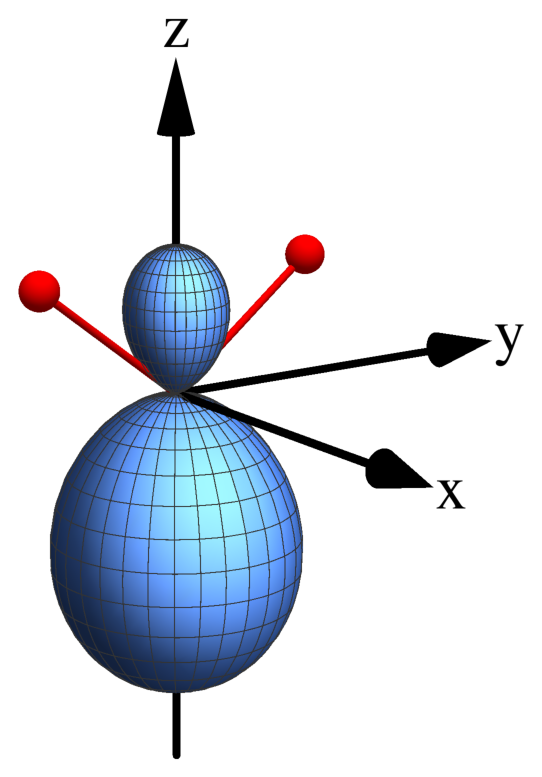
\includegraphics[width=\textwidth]{figures/ch_H2O/3a1/3a1extended.eps}
    \caption{Simplified $3a_{1}$ orbital}\label{fig:3a1_reduced}
  \end{subfigure}
  \,
  \begin{subfigure}[b]{0.25\linewidth}
    \centering
    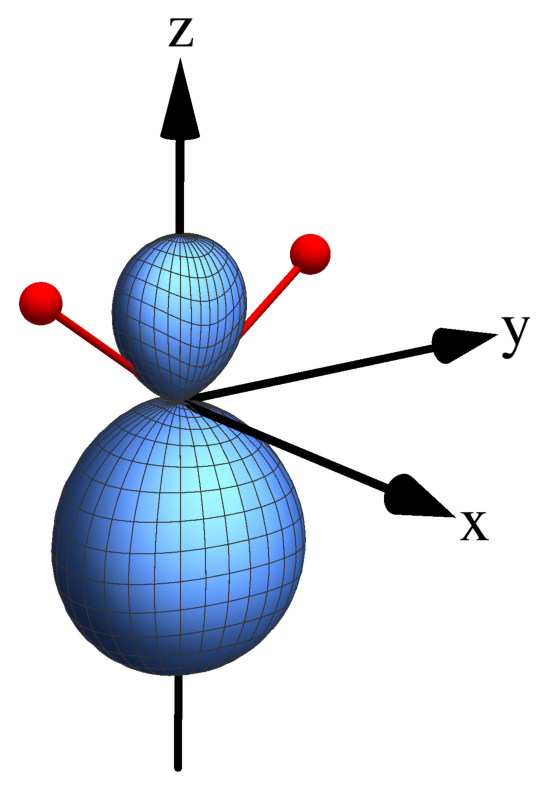
\includegraphics[width=\textwidth]{figures/ch_H2O/3a1/3a1Moccia.eps}
    \caption{Full Moccia $3a_{1}$ orbital}\label{fig:3a1_Moccia}
  \end{subfigure}
  \caption{Schematic display of the $3a_{1}$ molecular orbital (shown
    in blue along the $z$ axis) used to construct
    $V_{\mathrm{eff}}(r,\theta)$. The orbital obtained from a reduced
    expansion in \textsc{sto}s is shown in~(\ref{fig:3a1_reduced}),
    and the complete Moccia orbital is shown
    in~(\ref{fig:3a1_Moccia}). Also indicated (in red in the $y-z$
    plane) is the location of the protons. The $\hat{z}-$axis is the
    direction along which the external electric field of strength
    $F_{0}$ is applied.}
  \label{fig:3a1_prob_density}
\end{figure}

In order to illustrate the fraction of the full Moccia expansion that
our reduced wavefunction~(\ref{eq:3a1Moccia_expansion}) represents,
the projections of the probability densities over the $x-y$ plane are
shown as contours of constant density in
Figure~\ref{fig:3a1_xycontours}, for the height where the protons are
located. From the complete Moccia representation of the $3a_{1}$
\textsc{mo} (in dashed lines), one observes that the location of the
protons (shown as red circles) has an influence on the shape of the
upper lobe in the probability density, i.e., it introduces dependence
on the azimuthal angle $\varphi$. In our simplified expansion, where
only $l=0,1$ and $m=0$ symmetrical parts were included (shown with
solid lines), the probability density misses to represent the proper
azimuthal dependence that follows from the $m\neq 0$ parts.

\begin{figure}
  \centering
  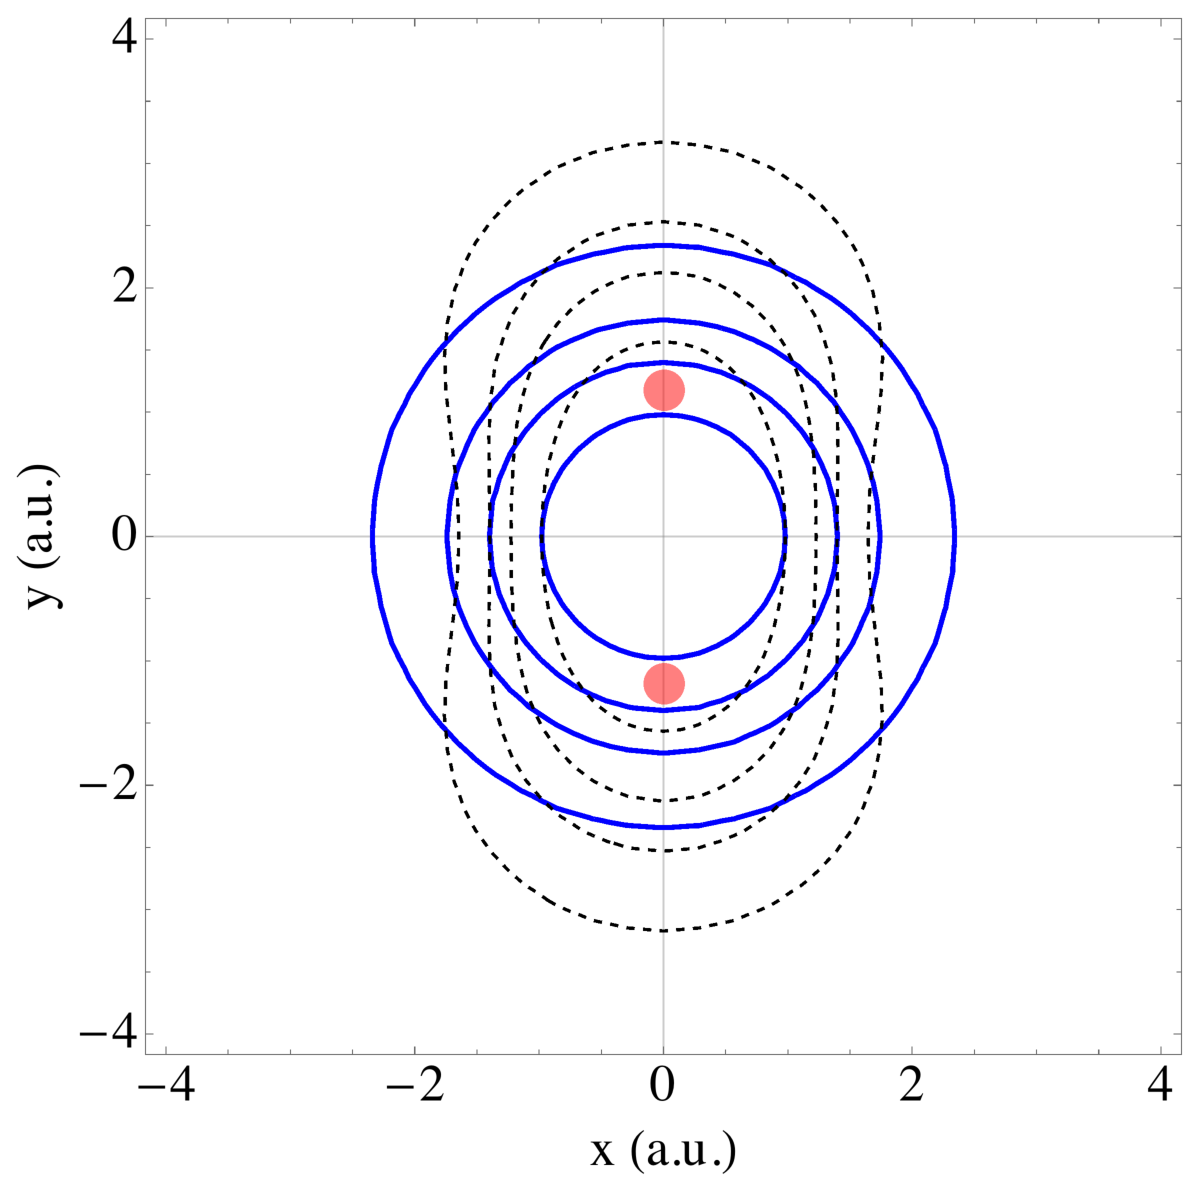
\includegraphics[width=0.6\textwidth]{figures/ch_H2O/3a1/orbitals3a1.eps}
  \caption{Projections of the probability densities for the $3a_{1}$
    orbital on the $x-y$ plane. The simplified \textsc{sto} expansion
    is indicated as continuous blue lines, and the full Moccia
    expansion is indicated as black dashed lines. The protons are also
    indicated as red circles. The chosen contour values are $0.5, 0.3,
    0.2, 0.1$ starting from the innermost contour.}
  \label{fig:3a1_xycontours}
\end{figure}

The non-spherical effective potential corresponding to the
\textsc{sto} expansion~(\ref{eq:3a1Moccia_expansion}),
$V_{\mathrm{eff}}(r,\theta)$, is obtained from the Schr\"{o}dinger
equation in spherical polar coordinates,
%
\begin{eqnarray}
  \left[ -\frac{1}{2} \nabla^{2} +
  V_{\rm{eff}}(r,\theta) \right] \psi_{3a_{1}}(r,\theta) =
  E_{3a_{1}} \psi_{3a_{1}}(r,\theta).
\label{eq:sch_eq3d}
\end{eqnarray}
%
For given $E_{3a_{1}}$ and $\psi_{3a_{1}}(r,\theta)$ it is
straightforward to solve~(\ref{eq:sch_eq3d}) for
$V_{\mathrm{eff}}(r,\theta)$. In order to use this potential to define
a Hamiltonian for the $3a_{1}$ orbital in an electric field, an
asymptotic Latter correction needs to be applied.

Other strategies for finding an effective potential could be pursued,
such as using a density functional, inserting the Moccia wavefunction,
and then performing an azimuthal angle average. Ultimately, one would
like to extend density functional theory~(\textsc{dft}) from finding
ground-state energies to obtaining resonance positions and
widths. This might be feasible using a combination of time-dependent
\textsc{dft} and Floquet theory. The goal of the present work is more
modest: we calculate the response of an isolated molecular orbital in
a simple approximation. Recently, the problem of small molecules in a
dc field has revealed the effect of electron-electron interactions on
Stark resonance parameters~\cite{ScrinziJPhysB_ECS}. It will be
interesting to observe such effects for the water molecule in future
work.


\subsection{Interpolation and Latter correction of the
  non-spherical effective potential}
\label{ch:3a1_Latter}

The non-central effective potential, $V_{\mathrm{eff}}(r,\theta)$,
leads no longer to an orbital of $(l,m)$ symmetry, i.e.,
$2p_{z}$. This reflects the geometry of the problem as a consequence
of the location of the protons. The use of this more general potential
implies that the Latter criterion~\cite{LatterCor_1955}, which ensures
the proper asymptotic behaviour of the potential, is not as
straightforward to implement as in the case of the spherical potential
discussed in Sec.~\ref{ch:1b1_1b2}, where the correction applies
beyond a determined $r$ value~\cite{sarias_2016}. In this case, the
correction must be implemented in the $r-\theta$ plane, by defining a
$\theta-$dependent boundary beyond which the potential obtained
from~(\ref{eq:sch_eq3d}) rises above $-1/r$ in the asymptotic
region~\cite{sarias_2017}.

The $\theta$ coordinate is fixed at two extreme positions, such as
$\theta = 0$ and $\theta = \pi$, in order to find the corresponding
$r$ values $r_{0}$ and $r_{\pi}$, for which
$V_{\mathrm{eff}}(r,\theta) = -1/r$ is satisfied, then we interpolate
between them by introducing the $\theta-$dependent function
%
\begin{eqnarray}
r_{\rm{match}}(\theta) & = & \bar{r} - (r_{\pi} - \bar{r}) \cos\theta,
\label{eq:rMatch}
\end{eqnarray}
%
where $\bar{r} = (r_{0} + r_{\pi})/2$. With this approach we redefine
the effective potential to be the non-central potential derived from
the reduced Moccia wavefunction using Equation~(\ref{eq:sch_eq3d})
when $r < r_{\mathrm{match}}(\theta)$, and $-1/r$ otherwise.

The weighted functions used to construct the Moccia
orbitals~\cite{Moccia_1964} imply a potential difficulty in our
problem. Since these functions are not exact solutions of the
Schr\"{o}dinger equation but were obtained from the variational
principle by implementing a self-consistent
calculation~\cite{Moccia_JCP_2164}, there may be regions in the
$(r,\theta)$ domain where $\psi_{3a_{1}}(r,\theta)$ vanishes, whereas
its second derivative remains finite; this produces a nodal line in
the electronic potential. Thus finding a potential for which our
approximate wavefunction satisfies a Schr\"{o}dinger equations
represents an intricate problem.

It turns out that the nodal region is so narrow that when solving the
Schr\"{o}dinger equation the kinetic energy term dominates and it is
possible to obtain a solution that remains close to that obtained by
the \textsc{hf} method~\cite{Moccia_1964}, regardless of the fact that
there is a region where the effective potential might diverge.

The probability density exhibits two humps indicating the positions of
the protons, which is consistent with
Figure~\ref{fig:3a1_prob_density}, and the effects of the mixing with
the $s-$state. One may argue that one of the reasons this nodal region
in the potential does not have a negative impact on the results is due
to the way the $3a_{1}$ orbital responds to the effective potential by
avoiding this region, its probability density being distributed as
shown in Figure~\ref{fig:density_contours}. A numerical interpolation
of $V_{\mathrm{eff}}(r,\theta)$ is implemented in order to ensure it
continues smoothly over this problematic region.

\begin{figure}
  \centering
  \begin{subfigure}[b]{0.245\linewidth}
    \centering
    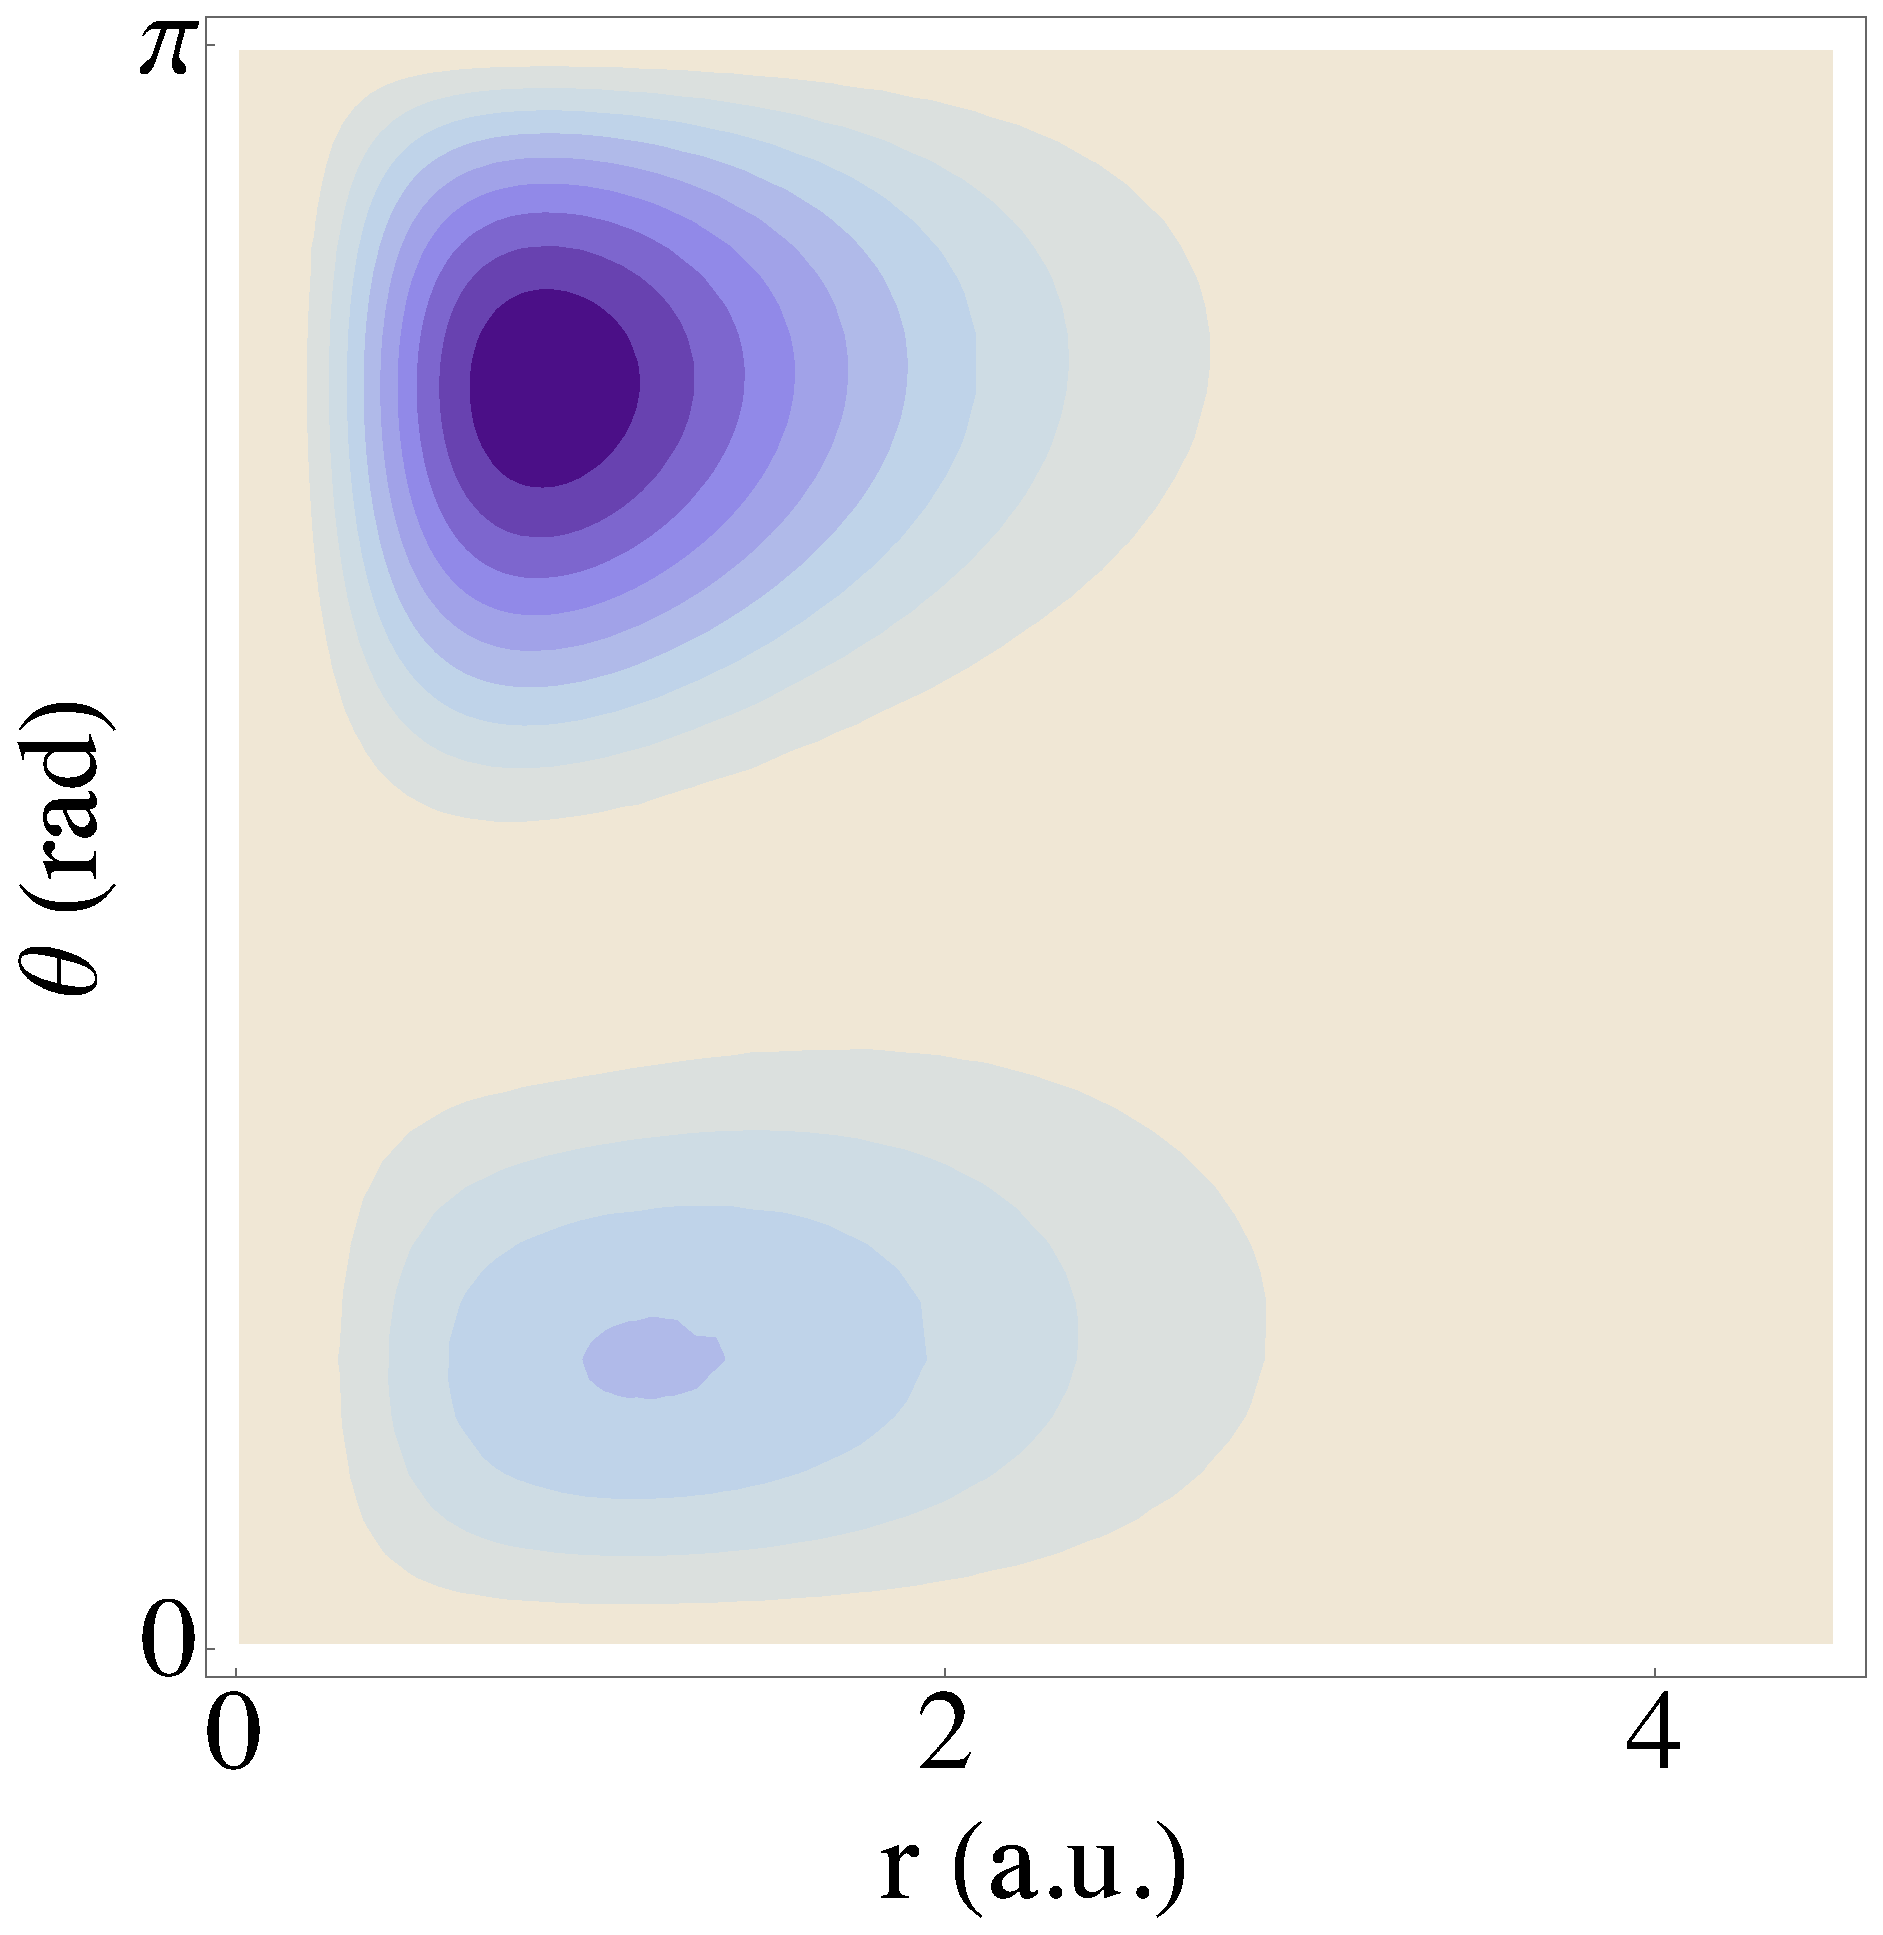
\includegraphics[width=\textwidth]{figures/ch_H2O/3a1/contour3a132s.eps}
    \caption{}\label{fig:Moccia32s}
  \end{subfigure}
  \,
  \begin{subfigure}[b]{0.275\linewidth}
    \centering
    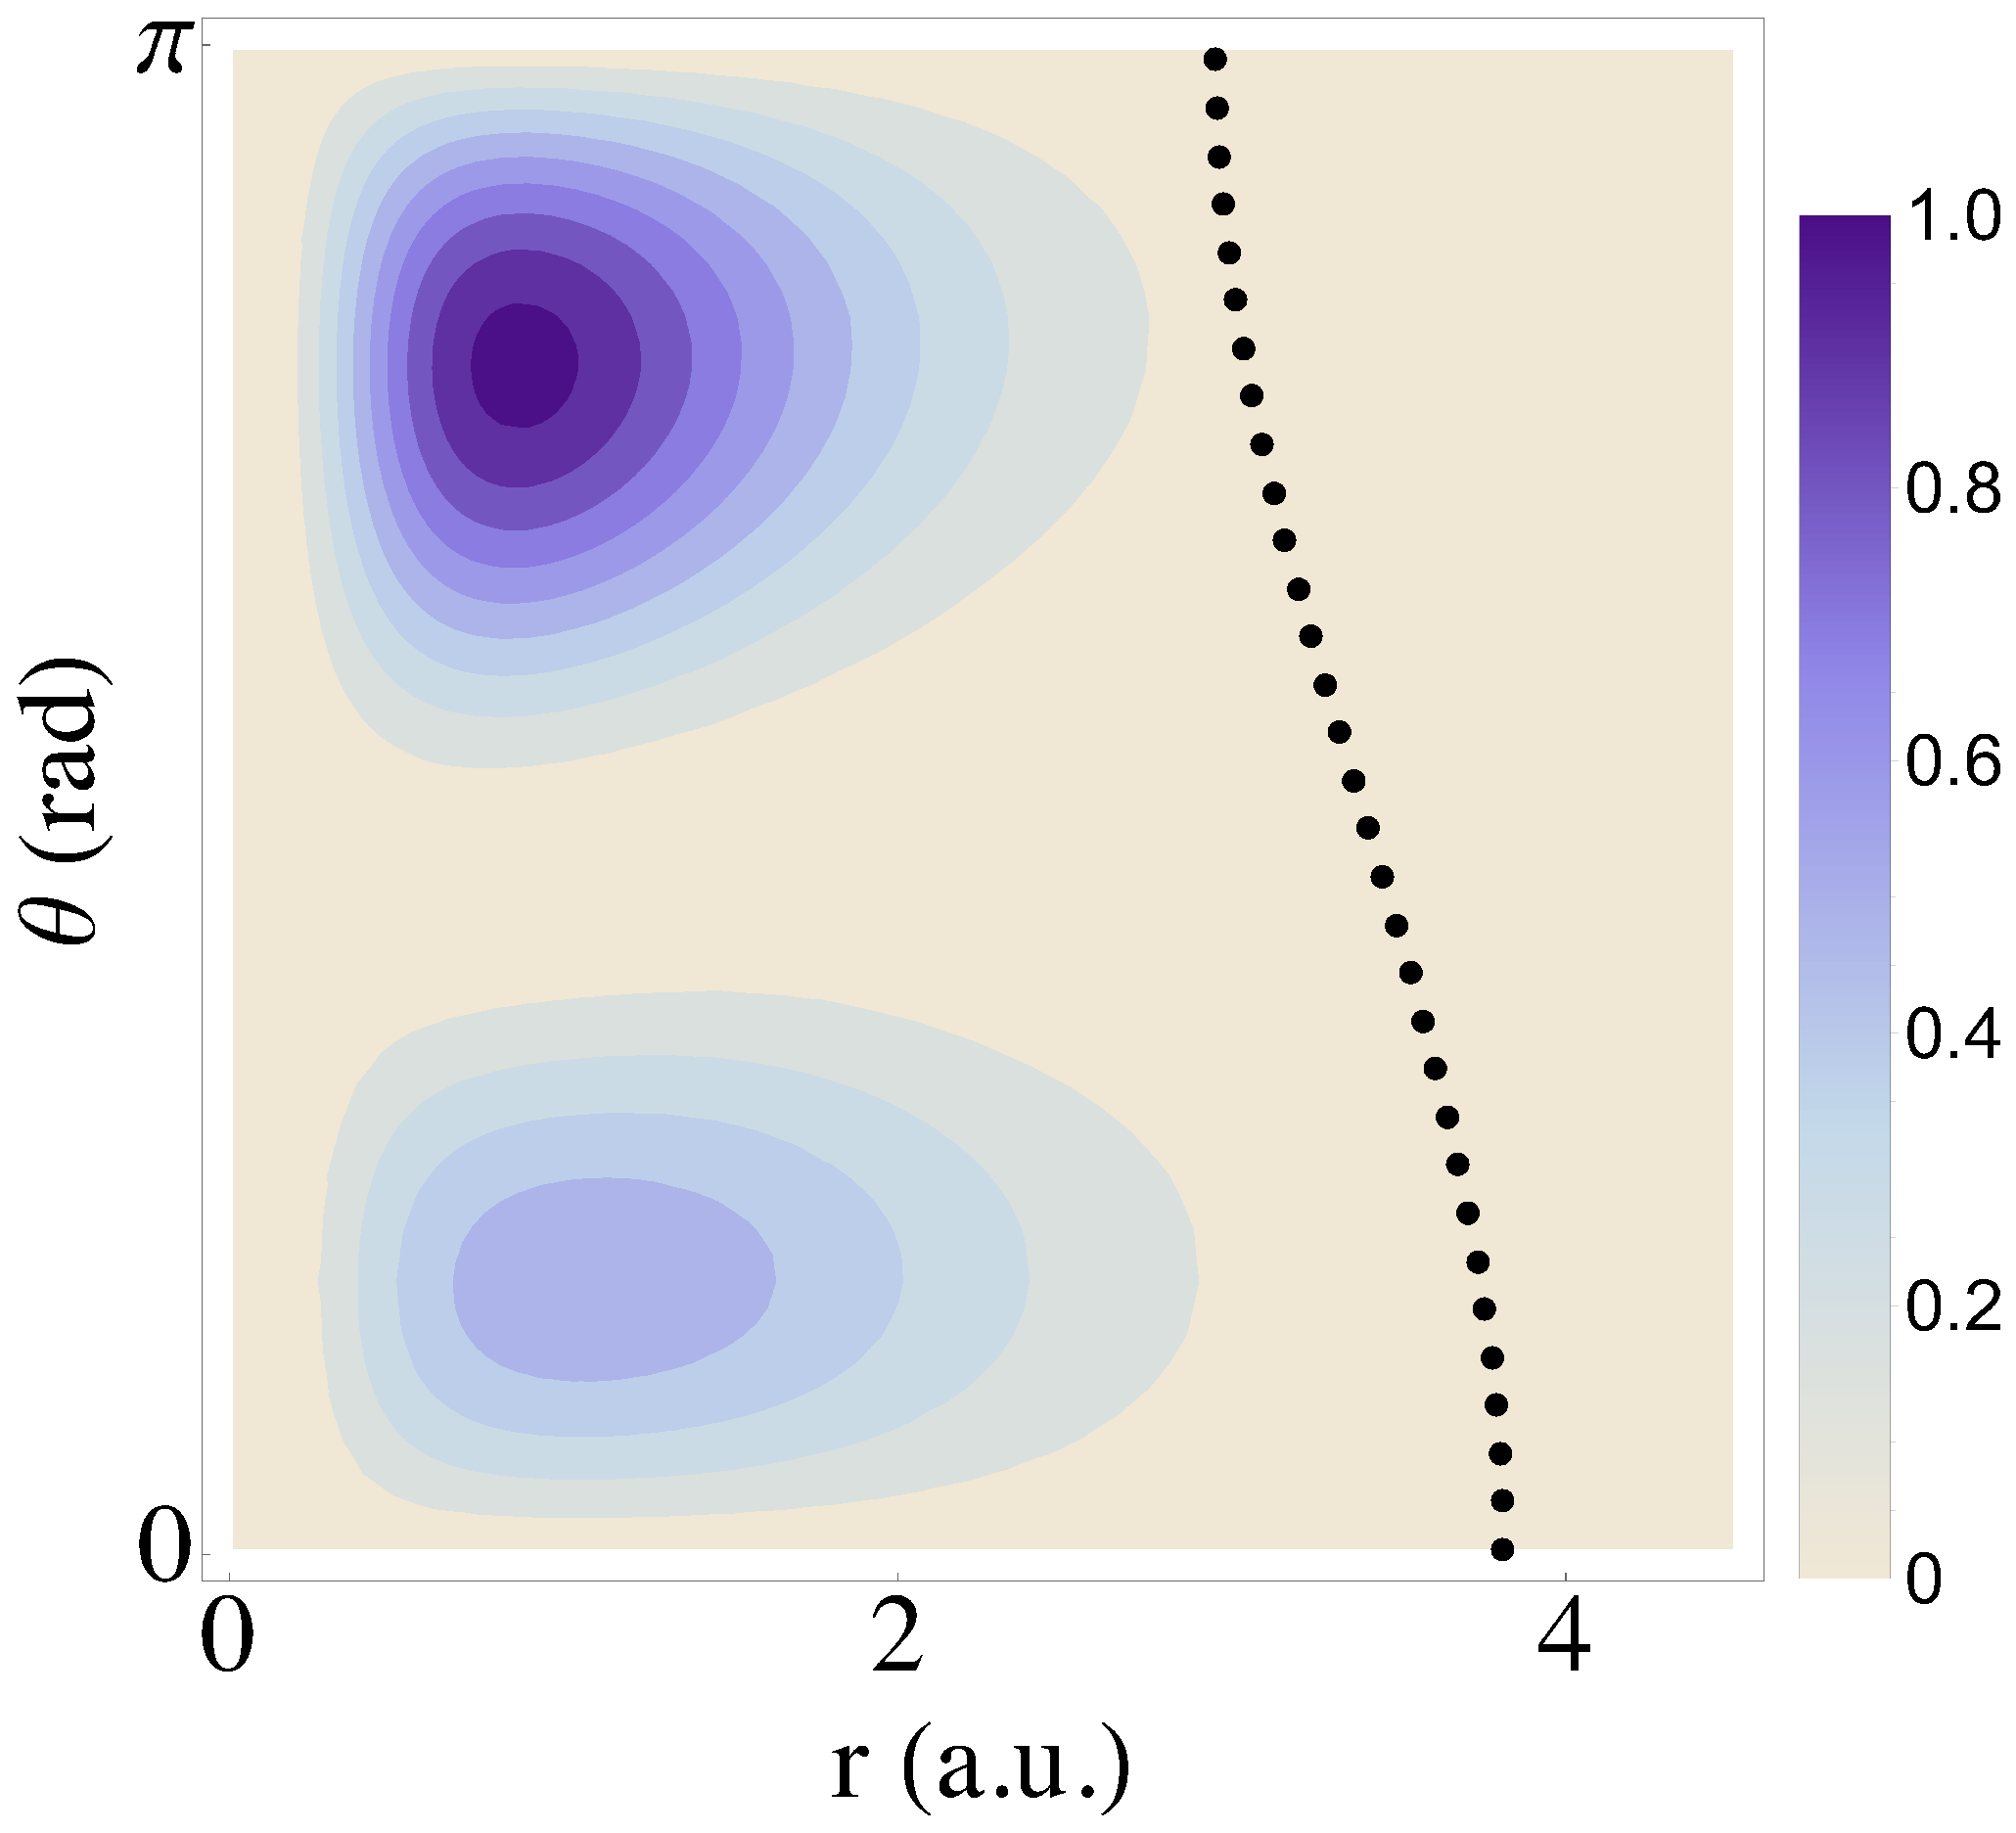
\includegraphics[width=\textwidth]{figures/ch_H2O/3a1/contour3a1intpl.eps}
    \caption{}\label{fig:intp32s}
  \end{subfigure}
  \caption{Contour plots of the scaled probability density,
    $|\psi_{\mathrm{3a_{1}}}|^{2}r^{2}\sin(\theta)/(2\pi)$, for the
    $3a_{1}$ molecular orbital. The orbital density constructed from
    the reduced \textsc{sto} expansion is shown
    in~(\ref{fig:Moccia32s}), while the solution obtained from the
    non-spherical $V_{\mathrm{eff}}(r,\theta)$ with Latter correction
    is shown in~(\ref{fig:intp32s}) along with a dotted line
    indicating where the Latter correction acts. Starting from the
    innermost contours the contour values are $0.45\dots 0.05$ for the
    upper density lobes and $0.2\dots 0.05$ for the lower density
    lobes, in steps of $0.05$.}
  \label{fig:density_contours}
\end{figure}

The interpolation is achieved by collecting data from the evaluation
of the potential on two sections of the $(r,\theta)$ grid in the
vicinity of the nodal line, where the potential evaluates to finite
values. Then, a numerical interpolation was carried out between those
regions in order to obtain a continuous function,
$V_{\mathrm{eff}}^{\mathrm{intp}}(r,\theta)$, on the two-dimensional
grid. The Latter correction is applied to the interpolated potential
and the effective potential is defined according to~(\ref{eq:rMatch}):
%
\begin{eqnarray}
  V_{\mathrm{eff}}(r,\theta) = \left\{
  \begin{split}
    V_{\mathrm{eff}}^{\mathrm{intp}}(r,\theta)\
    & \mathrm{~for} & r < r_{\mathrm{match}}(\theta) \\
    -1/r\ & \mathrm{~for} &  r > r_{\mathrm{match}}(\theta)
  \end{split}
\right.
\label{eq:latterVeff}
\end{eqnarray}
%

Figure~\ref{fig:Moccia32s} shows the probability density for the
$3a_{1}$ \textsc{mo} as a contour plot in the $r-\theta$ plane as
obtained from the reduced Moccia expansion in
\textsc{sto}s~(\ref{eq:3a1Moccia_expansion}). Figure~\ref{fig:intp32s}
shows the same for the solution of the Schr\"{o}dinger
equation~(\ref{eq:sch_eq3d}) using the interpolated
$V_{\mathrm{eff}}(r,\theta)$, defined in
Equation~(\ref{eq:latterVeff}), with the Latter
correction~\cite{LatterCor_1955} applied in the asymptotic $r-$region.

The effective potential~(\ref{eq:latterVeff}) results in the
probability density shown in Figure~\ref{fig:intp32s} and yields an
orbital energy of $-0.5579\ \mathrm{a.u.}$ for the $3a_{1}$
\textsc{mo}, with a relative change of $0.32\%$ in comparison with the
self-consistent result of Moccia~\cite{Moccia_1964} of
$-0.5561\ \mathrm{a.u.}$.

As Figure~\ref{fig:intp32s} indicates, the implementation of the
Latter correction to the orbital-dependent potential obtained from
Equation~(\ref{eq:sch_eq3d}) introduces a slight re-adjustment of the
density, with a somewhat higher probability density in the region $0 <
\theta < \pi/2$. The probabilities for finding the electron at $\pi/2
< \theta < \pi$ is $66.2\%$ before the Latter correction is applied
(Figure~\ref{fig:Moccia32s}) and becomes $63.5\%$ for the case shown
in Figure~\ref{fig:intp32s}.

\subsection{Exterior complex scaling}
\label{ch:3a1_ecs}

For our aim of computing the resonance parameters that describe the
tunneling process, a modified exterior complex scaling to the radial
coordinates was implemented. As was described in
Sec.~\ref{ch:ecs_1b11b2}, the $r-$coordinate is extended into the
complex plane by the phase function $\chi(r)$,
Eq.~(\ref{eq:ecs_theta}), with $r$ replaced by $r^{*} =
r\exp[i\chi(r)]$. The phase function $\chi(r)$ is chosen to be very
small for $r$ values smaller than the Latter radius $\bar{r}$. It then
turns on from nearly zero to reach an asymptotic value
$\chi_{\mathrm{s}}$ at $r-$values just outside where the Latter
correction is applied, i.e., $r_{\mathrm{s}} > r_{\mathrm{match}}$. In
such a way as to provide exterior complex scaling without a hard
radius at which a derivative discontinuity would have to be
applied~\cite{ecsScrinzi}.

A non-Hermitian Hamiltonian results from considering the additional
terms that the modified complex scaling to the radial coordinates
introduces in the Schr\"{o}dinger equation. The complex wavefunction
is separated into real and imaginary parts, $\psi_{R(I)}$, such that
the problem of describing the ionization regime of the $3a_{1}$
\textsc{mo} under an external dc field applied along the orientation
axis of the orbital is expressed in terms of a system of partial
differential equations for the real and imaginary parts of
$\widetilde{\psi}(r,\theta)$ in spherical polar coordinates given
explicitly as Eq.~(\ref{eq:pde_system}). Schematically, the equations
are extensions of the field-free Schr\"{o}dinger
equation~(\ref{eq:sch_eq3d}) and $\widetilde{\psi}(r,\theta)$
satisfies~\cite{sarias_2017}
%
\begin{eqnarray}
  \begin{split}
    \left[ -\frac{1}{2}\nabla^{2} + V_{\mathrm{eff}}(r,\theta)
      \pm F_{0}z \right] \widetilde{\psi} = (E_{R} - i\Gamma/2)
    \widetilde{\psi},
  \end{split}
  \label{eq:sch_tunneling_params}
\end{eqnarray}
%
where $E_{R}$ is the resonance position and $\Gamma$ the
width. Compared to Eq.~(\ref{eq:sch_eq3d}), the Hamiltonian in
Eq.~(\ref{eq:sch_tunneling_params}) contains the interaction with the
external field and complex scaling is responsible for the replacement
$E_{3a_{1}} \to E_{R} - i\Gamma/2$; while $\widetilde{\psi}$ remains
square integrable.

The domains of $r$ and $\theta$ values are restricted to the intervals
$r\in[\epsilon, r_{\mathrm{max}}]$ and $\theta\in[\eta,\pi-\eta]$,
with typical values $\epsilon = 10^{-2}\ \mathrm{a.u.}$, $\eta =
10^{-2}$, $r_{\mathrm{max}} = 28\ \mathrm{a.u.}$ In the limit of low
field strengths, i.e., $F_{0} = 0.05, 0.06$, the value of
$r_{\mathrm{max}}$ was increased to $40\ \mathrm{a.u.}$ in order to
ensure the outer turning points lie inside the grid, as the tunneling
barrier extends to larger $r$.

The problem of finding a solution of the Schr\"{o}dinger equation for
the $3a_{1}$ \textsc{mo} with contributions of $2s$ and $2p-$type
states requires a set of boundary conditions that describes the
properties of the orbital on the grid. In contrast with the $m = \pm
1$ solutions obtained for the $1b_{1}$ and $1b_{2}$ \textsc{mo}s of
H$_{2}$O~\cite{sarias_2016}, Neumann boundary conditions are
implemented for the angular coordinate $\theta$ in order to obtain an
eigenstate and orbital energy consistent with the variational
results~\cite{Moccia_1964}. This choice of boundary conditions, that
the derivative with respect to $\theta$ vanishes at the limits of the
mesh $(\theta = 0 ~\mathrm{and}~ \theta = \pi)$, leads to solutions
$\psi_{R(I)}(r,\theta)$ with a probability density consistent with the
$\theta-$dependence of the $3a_{1}$ orbital, as shown in
Figure~\ref{fig:density_contours}.



\section{Partial-wave method with a complex absorbing potential}
\label{ch:partial_wave}
% describe method, problem to solve and implementation of the
% formalism




% NEXT SECTION
%The physical parameters of interest, namely the resonance position,
%$E_{R}$, and width, $\Gamma = -2E_{I}$, that characterize the
%tunneling process of the quasi-stationary state when an external
%electric dc field is applied along the $\pm\hat{z}$ directions, were
%found by solving the system of partial differential equations
%(Ref.~\cite{PhysRevA.94.053413}) for a set of field strength values,
%$F_{0}$, as if it were an inhomogeneous problem. In the vicinity of a
%location in the $(r,\theta)$ plane where the probability amplitude is
%expected to be large, a two-parameter root search was implemented to
%determine $\{E_{R},E_{I}\}$, the complex energy that maximizes the
%probability density amplitude in the $2d-$grid.



\section{Stark resonance parameters}
\label{ch:stark_params}

In the following subsections we present plots of the physical
parameters of interest, namely the resonance position, $E_{R}$, and
width, $\Gamma = -2E_{I}$, that characterize the tunneling process of
the quasi-stationary state when an external electric dc field is
applied along the $\pm\hat{z}$ directions. The system of partial
differential equations~(\ref{eq:pde_system}) is solved for a set of
field strength values, $F_{0}$, as if it were an inhomogeneous
problem. In the vicinity of a location in the $(r,\theta)$ plane in
which the probability amplitude is expected to be large, a
two-parameter root search is implemented in order to determine
${E_{R}, E_{I}}$, the complex energy that maximizes the probability
density amplitude in the $2d-$grid.

We explored the influence of a set of parameters involved in the
two-dimensional problem~(\ref{eq:pde_system}) on the eigenvalue
$E_{R}+iE_{I}$ which describes the ionization process as an
exponential decay in time in terms of resonance position and
half-width. In addition to testing the code against known results for
atomic hydrogen~\cite{Telnov_1989}, we have performed systematic
studies of our results for the H$_{2}$O orbitals against a number of
parameters in order to assess the accuracy of these results. One
parameter concerns the limiting resolution with which the
finite-element method proceeds (the \textsc{maxcellsize} parameter in
the \emph{Mathematica}~10 implementation of \textsc{ndsolve}, which we
call $\Delta$). For values $\Delta<0.02\ \rm{a.u.}$ we find stability
in the eigenvalues (real and imaginary parts) of two-three significant
digits. For the results quoted in Secs.~\ref{ch:1b1_1b2_results}
and~\ref{ch:3a1_results}, we then applied the more stringent criterion
of $\Delta=0.01\ \rm{a.u.}$

The second parameter which was investigated is the range where the
complex scaling function sets in, i.e., $r_{s}$ and $\Delta r$ in
Eq.~(\ref{eq:ecs_theta}). For the scaling method to work we require
scaling to set in for $r > r_0$ when the effective potential represents
a simple Coulomb tail, which in practice is satisfied by
$r_{s} > 2r_{0}$. We also need $\Delta r < 2\ \rm{a.u.}$ to guarantee
smooth turn-on in this region. Small values of $\Delta r$ pose
challenges for the automated finite-element method, since in the limit
of $\Delta r \to 0$ one would need to implement the derivative
discontinuity in the solution as discussed by
Scrinzi~\cite{ecsScrinzi}. We find stable results for the real and
imaginary parts of the eigenenergies at the level of three significant
digits for the range $10 < r_{s} < 15\ \rm{a.u.}$ Larger values would
require an increase in the computational domain beyond
$r=20\ \rm{a.u.}$

Finally, another systematic that was explored is the choice of the
ultimate scaling angle reached at large $r$, namely the value of
$\chi_{\rm{s}}$ in~(\ref{eq:ecs_theta}). For an accuracy demand of
three significant digits, and the other parameters chosen in the
ranges described above stability in the resonance widths is achieved
for $0.6< \chi_{\rm{s}} < 1.2$ rad.


\subsection{$1b_{1}$ and $1b_{2}$ molecular orbitals}
\label{ch:1b1_1b2_results}

% include the plots that the first 3 paragraphs in secIII(PRA2016)
% refer to about the systematic studies of the relevant parameters for
% the calculation

\begin{figure}
  \centering
  \includegraphics[width=0.7\textwidth]{figures/ch_H2O/1b1_1b2/resPositionvsF1b11b2.eps}
  \caption{Resonance position as a function of the external field
    strength $F_{0}$ for the $1b_{1}$ (red circles) and $1b_{2}$ (blue
    triangles) \textsc{mo}s of H$_{2}$O.}
  \label{fig:1b11b2_position}
\end{figure}

\begin{figure}
  \centering
  \includegraphics[width=0.7\textwidth]{figures/ch_H2O/1b1_1b2/resWidthvsF1b11b2H1s.eps}
  \caption{Resonance width as a function of the external field
    strength $F_{0}$ for the $1b_{1}$ (red circles) and $1b_{2}$ (blue
    triangles) \textsc{mo}s of H$_{2}$O. For comparison, atomic
    hydrogen H$(1s)$ ionization rates from
    Refs.~\cite{Telnov_1989,Kolosov_1987} are shown as crosses.}
  \label{fig:1b11b2_width}
\end{figure}

Figure~\ref{fig:1b11b2_position} shows the resonance position $E_{R}$
as obtained from the present calculations for the weakly bound
$1b_{1}$ and the strongly bound $1b_{2}$ valence orbitals as a
function of applied electric field strength $F_{0}$. In the limit of
zero field the calculation reproduces the \textsc{scf} eigenvalues of
Moccia~\cite{Moccia_1964}. The field has to be strong (in comparison
with atomic hydrogen results for $2p$ orbitals~\cite{Telnov_1989}) in
order to change the resonance position appreciably. For the more
deeply bound $1b_{2}$ orbital the shift in resonance position
saturates with field strength.

In Figure~\ref{fig:1b11b2_width} the resonance widths are shown for
both orbitals as functions of external field strength $F_{0}$. The
graphs display threshold behavior at the weaker field strengths. As
expected, we find a lower threshold (critical field strength) for the
more weakly bound $1b_{1}$ orbital. Interestingly, however, at a field
strength of about $F_{0} = 0.3\ \mathrm{a.u.}$ the values for the
widths cross; that is, the deeper bound $1b_{2}$ orbital displays a
larger ionization rate as the field strength is increased further.

Also shown in Figure~\ref{fig:1b11b2_width} are the widths for the
H($1s$) orbital from Refs.~\cite{Telnov_1989,Kolosov_1987}. They can
be compared to the $1b_{1}$ orbital results, since the binding energy
is very close in the free-field limit. Since the tunneling barrier is
mostly in the asymptotic regime where the potential energy has a
$-1/r$ tail, it is not surprising that the widths for
H$_{2}$O($1b_{1}$) and H($1s$) share some similarity in shape. In the
tunneling region H($1s$) has an ionization rate that is larger by
about an order of magnitude. In the over-barrier regime, however, the
ionization rates come to within a factor of 3. Reasons for why the
$1b_1$ water molecular orbital is harder to ionize than H($1s$) have
to do with the different shape of the orbital density ($m=1$ \emph{vs}
the spherical H($1s$) density), and the substantially more attractive
potential at shorter distances.

An examination of contour plots of the densities $\Psi^{*}\Psi$, as
well as of the potential energies $V_{\mathrm{eff}} - F_{0}z$ for
different field strengths (both as a function of $r,\theta$), allows
us to make the following observations. For field strengths $F_{0} <
0.1\ \mathrm{a.u.}$ there is a barrier the electrons need to penetrate
in order to be ionized. From the potential-energy plot shown in
Figure~\ref{fig:1b11b2_position} one can see that for weak fields
(small values of $F_{0}$) the barrier is longer for the more deeply
bound $1b_{2}$ orbital. This explains why the ionization threshold
occurs for $F_{0} > 0.1\ \mathrm{a.u.}$ for this orbital, which is
about a factor of $2$ larger than for the $1b_{1}$ orbital.

The field-strength region where the ionization rates (resonance
widths) display a change in character, i.e., turn over to rise much
more gradually with the field strength $F_{0}$, can be characterized
as a regime where there is a narrow potential saddle at small $\theta$
in the vicinity of $r \approx 3\ \mathrm{a.u.}$, such that electron
flux can leave and is then accelerated by the electric field. The
crossing of the ionization rates for the $1b_{1}$ and $1b_{2}$
orbitals occurs since the saddle in the potential becomes effectively
lower at strong fields for the $1b_{2}$ orbital. This can be inferred
from the comparison of the two effective potentials, which share the
same asymptotic behaviour beyond $r = 4.3\ \mathrm{a.u.}$ (see
Figure~\ref{fig:Veff1b11b2}).

The origin for the different radial dependencies of the effective
potential for the two orbitals can be found in the geometry of the
water molecule. The weakly bound $1b_{1}$ orbital has its lobes
perpendicular to the plane defined by the location of the three
nuclei. Therefore, it is least affected by the two protons. The
$1b_{2}$ orbital explores the potentials due to the protons more
strongly in the \textsc{scf} calculation of Moccia, and therefore, the
resulting $V_{\mathrm{eff}}(r)$ has a more attractive region in the
range $0.7\ \mathrm{a.u.} < r < 4.3\ \mathrm{a.u.}$.

%The numerical results are summarized in Table~\ref{tab:1b11b2_results}
%for further reference, i.e., for future comparisons with calculations
%based on other models for the molecular orbitals.

%\begin{table}[t]
%\centering
%\caption{\label{tab:1b11b2_results} Resonance positions and widths for
%  different field strengths (in atomic units). The numbers in
%  parentheses indicate the exponent $k$; that is, the numbers are to
%  be multiplied by $10^{k}$.}
%\begin{tabular}{rrrrr}
%\toprule
% & & $1b_{1}$ & & $1b_{2}$ \\
%$F_{0}$ & $E_{R}$ & $\Gamma$ & $E_{R}$ & $\Gamma$ \\
%\midrule
%$0.1$ & $-0.506$ & $1.14(-3)$ & $-0.689$ & $4.04(-5)$ \\
%$0.2$ & $-0.525$ & $2.28(-2)$ & $-0.718$ & $1.23(-2)$ \\
%$0.3$ & $-0.546$ & $6.74(-2)$ & $-0.760$ & $7.51(-2)$ \\
%$0.4$ & $-0.564$ & $1.24(-1)$ & $-0.790$ & $1.91(-1)$ \\
%$0.5$ & $-0.580$ & $1.90(-1)$ & $-0.796$ & $3.11(-1)$ \\
%$0.6$ & $-0.593$ & $2.61(-1)$ & $-0.797$ & $4.11(-1)$ \\
%\bottomrule
%\end{tabular}
%\end{table}


\subsection{$3a_{1}$ molecular orbital}
\label{ch:3a1_results}

The numerical results from applying the procedure described in
Section~\ref{ch:3a1} are shown in Figures~\ref{fig:3a1_position}
and~\ref{fig:3a1_width}.

\begin{figure}
  \centering
  \includegraphics[width=0.7\textwidth]{figures/ch_H2O/3a1/resPosvsForbitals_compf32snew.eps}
  \caption{Resonance position in atomic units as a function of the
    external field strength $F_{0}$ and the orientation of the field,
    along the $\pm\hat{z}$ direction (red triangles/blue circles), for
    the $3a_{1}$ \textsc{mo} of H$_{2}$O. As a reference, the resonance
    position values for the $1b_{1}$ (dashed line) and $1b_{2}$
    (dot-dashed line) \textsc{mo}s are also included.}
  \label{fig:3a1_position}
\end{figure}

\begin{figure}
  \centering
  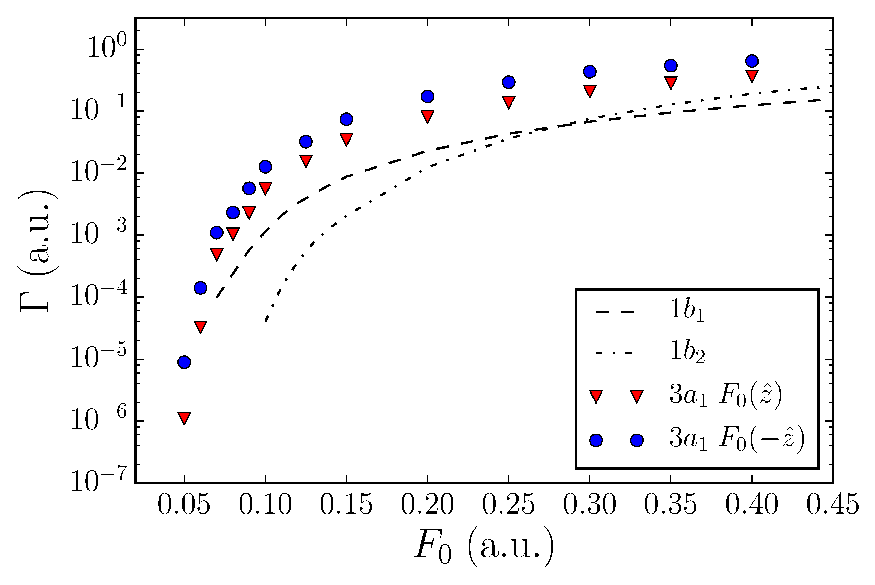
\includegraphics[width=0.7\textwidth]{figures/ch_H2O/3a1/resWidthvsForbitals_compf32snew.eps}
  \caption{Resonance width in atomic units as a function of the
    external field strength $F_{0}$ and the orientation of the field,
    along the $\pm\hat{z}$ direction (red triangles/blue circles), for
    the $3a_{1}$ \textsc{mo} of H$_{2}$O. For reference, the resonance
    widths for the $1b_{1}$ (dashed line) and $1b_{2}$ (dot-dashed
    line) \textsc{mo}s are also shown.}
  \label{fig:3a1_width}
\end{figure}

The resonance positions $E_{R}$ are shown in
Figure~\ref{fig:3a1_position} for external fields applied along the
$\pm\hat{z}$ directions (red triangles/blue circles) for a range of
external field strengths. For reference, the resonance positions
obtained for the $1b_{1}$ and $1b_{2}$ \textsc{mo}s using a
spherically symmetric potential, $V_{\mathrm{eff}}(r)$, are also
indicated in the form of dashed and dot-dashed lines respectively. For
zero field strength $F_{0} = 0$ self-consistent eigenenergies obtained
by Moccia~\cite{Moccia_1964} are included as black crosses for the
three valence orbitals of interest. As expected, the resonance
position for the $3a_{1}$ orbital is bracketed by those for the
$1b_{1}$ and $1b_{2}$ orbitals.

It can be noticed that for external fields applied along the
$-\hat{z}$ direction, where most of the density is located, the field
strength $F_{0}$ has to be strong, i.e., $F_{0}>0.1\ \mathrm{a.u.}$,
for the resonance position to change appreciably. On the other hand,
the resonance position for fields applied along $+\hat{z}$ appears to
be more sensitive at weaker fields. However the barrier appears to be
longer for external fields applied along the $+\hat{z}$ direction, at
a field strength of about $F_{0} = 0.2\ \mathrm{a.u.}$ the position
values cross, indicating a higher sensitivity of the resonance
positions for fields applied along the negative $\hat{z}$ direction as
the field strength is increased further.

Figure~\ref{fig:3a1_width} shows the resonance widths corresponding to
external fields applied along the $\pm\hat{z}$ directions, as a
function of the field strength $F_{0}$. The results obtained with a
symmetric effective potential, $V_{\mathrm{eff}}(r)$, for the $1b_{1}$
and $1b_{2}$ \textsc{mo}s are also shown as dashed and dot-dashed
lines for comparison purposes.

In analogy to the $m=\pm 1$ orbitals, the ionization rates for the
$3a_{1}$ \textsc{mo}, associated with the lifetime of the decaying
state via $\Gamma\tau=1$, exhibit a threshold behaviour at the weaker
field strengths. Interestingly, for the two directions of the applied
field, we find a lower critical field strength for the $3a_{1}$
orbital in comparison to what the more weakly bound orbital, $1b_{1}$,
indicates.  In the tunneling region, the $3a_{1}$ orbital for fields
applied along the $-\hat{z}$ direction (blue squares) shows an
ionization rate that is about one order of magnitude larger than the
ionization rate for fields applied in the opposite direction (red
triangles), this gap becomes narrower as the field strength increases
toward the over-barrier regime.

The numerical results for the H$_{2}$O valence orbitals studied in
this chapter, $1b_{1}$, $1b_{2}$ and $3a_{1}$, are summarized in
Table~\ref{tab:3a1_results} for further reference, i.e., to allow
comparison with future calculations based on other models for the
molecular orbitals.


\begin{table}[t]
\centering
\caption{\label{tab:3a1_results} Resonance positions and widths for
  different field strengths (in atomic units). The orientation of the
  external field is indicated by $\pm\hat{z}$. The numbers in
  parentheses indicate the exponent $k$, so that the numbers are
  multiplied by $10^{k}$.}
\begin{tabular}{rrrrrrrrr}
\toprule
&& $3a_{1}(\hat{z})$ && $3a_{1}(-\hat{z})$ && $1b_{1}$ && $1b_{2}$ \\
\midrule
$F_{0}$&$E_{R}$&$\Gamma$&$E_{R}$&$\Gamma$&$E_{R}$&$\Gamma$&$E_{R}$&$\Gamma$ \\
\midrule
$0.05$ &   --~~ &$1.09(-6)$&$-0.556$&$8.91(-6)$ & --~~ & --~~ & --~~ & --~~ \\
$0.06$ &   --~~ &$3.23(-5)$&$-0.556$&$1.41(-4)$ & --~~ & --~~ & --~~ & --~~ \\
$0.07$ &$-0.582$&$4.82(-4)$&$-0.557$&$1.09(-3)$&$-0.502$&$9.82(-5)$ & --~~ & --~~ \\
$0.08$ &$-0.587$&$1.03(-3)$&$-0.559$&$2.31(-3)$&$-0.503$&$2.38(-4)$ & --~~ & --~~ \\
$0.09$ &$-0.594$&$2.26(-3)$&$-0.568$&$5.65(-3)$&$-0.504$&$5.72(-4)$ & --~~ & --~~ \\
$0.1$  &$-0.600$&$5.53(-3)$&$-0.573$&$1.26(-2)$&$-0.506$&$1.14(-3)$&$-0.689$&$4.04(-5)$\\
$0.125$&$-0.617$&$1.54(-2)$&$-0.589$&$3.21(-2)$&$-0.510$&$3.76(-3)$&$-0.694$&$5.45(-4)$\\
$0.15$ &$-0.635$&$3.41(-2)$&$-0.607$&$7.39(-2)$&$-0.515$&$8.73(-3)$&$-0.701$&$2.04(-3)$\\
$0.2$  &$-0.668$&$7.98(-2)$&$-0.656$&$1.72(-1)$&$-0.525$&$2.28(-2)$&$-0.718$&$1.23(-2)$\\
$0.25$ &$-0.698$&$1.37(-1)$&$-0.708$&$2.92(-1)$&$-0.536$&$4.33(-2)$&$-0.739$&$3.61(-2)$\\
$0.3$  &$-0.724$&$2.07(-1)$&$-0.796$&$4.31(-1)$&$-0.546$&$6.74(-2)$&$-0.760$&$7.51(-2)$\\
$0.35$ &$-0.747$&$2.81(-1)$&$-0.859$&$5.40(-1)$&$-0.555$&$9.46(-2)$&$-0.778$&$1.27(-1)$\\
$0.4$  &$-0.765$&$3.60(-1)$&$-0.957$&$6.40(-1)$&$-0.564$&$1.24(-1)$&$-0.790$&$1.91(-1)$\\
\bottomrule
\end{tabular}
\end{table}



%%% Local Variables:
%%% mode: latex
%%% TeX-master: "thesis"
%%% End:

\chapter{Above threshold ionization in laser-atom and laser-molecule interactions}
\label{cha:ati}

% mention:
%
% -ATI models, keldysh approach pionnering work with the strong field
% approximation
% -QM generalization including rescattering
% -study of the ATI spectrum following the one introduced by kopold

The phenomenon of above threshold ionization~\cite{ATI1979} has been
tackled through diverse approaches, attempts to find numerical
solutions to the time-dependent Schr\"{o}dinger equation
(TDSE)~\cite{muller_tdse1999,scrinzi_tdse1999,Joachain2000} lie among
the earliest ones. A variety of efforts that deal with the complexity
of solving this challenging numerical problem have been successful in
the past. In the same way, complementary approaches to the solution of
the TDSE, such as the so-called Volkov-based
methods~\cite{Faisal_1973,Reiss_1980,Kaminski_1997}, have revealed
their strengths within strong-laser field problems in which a
numerical solution would involve a computationally taxing problem. The
strong-field approximation~\cite{KeldyshSFA}, which lies among these
approaches and considers the binding potential as a perturbation, is
the foundation to the formalism discussed in this chapter.

Sec.~\ref{sec:keldysh} presents an overview of the pioneering work by
Keldysh which introduces the strong-field approximation to describe
the laser ionization of atoms. Next, a generalized approach that
introduces rescattering of the electron back to the vicinity of the
binding potential is included in Sec.~\ref{kopold_sfa}. The ionization
regime of a model He atom under a strong laser field is explored in
Sec.~\ref{sec:kopold_qm} for both scenarios: considering only direct
electrons where the ionization spectrum is reproduced by the Keldysh
amplitude, and using a compact expression for the transition amplitude
that encloses the limiting case of direct trajectories while allowing
electrons to rescatter to the parent ion as well. Additionally, this
study is extended to explore the laser ionization of the $1b_{1}$ and
$1b_{2}$ molecular orbitals of H$_{2}$O in Sec.~\ref{sec:mo_sfa}. The
analysis presented in this chapter closely follows that
of~\cite{Kopold_1997sfa}.



%In addiion to exploring the ionization regime of the He atom in
%Sec.~\ref{sec:kopold_qm}, laser ionization of the $1b_{1}$ and
%$1b_{2}$ molecular orbitals of H$_{2}$O is discussed in
%Sec.~\ref{sec:mo_sfa}.


\section{\label{sec:keldysh} Keldysh formalism}
% cjp on keldysh formalism (sec 2 and 3)

% pra56 becker, lewenstein

% eventually obtain keldysh amplitude, after using the two main
% approximations that lead to eq.7 in pra55 kopold


Theoretical models that describe the interaction between intense laser
fields and atoms go back to Keldysh theory of strong field
approximation. The theoretical framework for the strong-field
approximation introduced by Keldysh properly accounts for multiphoton
ionization and tunneling ionization, which establish two limiting
cases of strong-field ionization, and produced good agreement with
experimental data of electron spectra of ATI for relatively low
energies~\cite{Walker_1994exp}. In this chapter we are concerned with
the numerical evaluation of an improved Keldysh
approximation~\cite{Kopold_1997sfa} that accounts for rescattering and
reveals the complex structure of the ionization spectrum.

The transition amplitude from the ground state of an atom with binding
potential $V(\mathbf{r})$, before the arrival of the laser pulse, into
the scattering state $|\psi_{\mathbf{p}}(t)\rangle$ after the pulse
has passed is given by
\begin{eqnarray}
\label{eq:matrix_element}
\begin{split}
M_{\mathbf{p}} & = & \lim_{t\to\infty,t'\to -\infty}
{\langle \psi_{\mathbf{p}}(t) | U(t,t') | \psi_{0}(t') \rangle}.
\end{split}
\end{eqnarray}
Here it is assumed that in the limit of early times, $t'\to -\infty$,
the exact wave function reduces to the unperturbed wave function
$\psi_{0}(t)$ of the initial ground state. The time-evolution operator
$U(t, t')$ is the solution to the initial-value problem
\begin{eqnarray}
\label{eq:time_evolution}
\begin{split}
\left[ i\partial_{t} - H(t)
\right] U(t,t') = 0,& & U(t',t') = 1,
\end{split}
\end{eqnarray}
and propagates the wave function $|\psi(t)\rangle$ from $t'$ to $t$
under the full Hamiltonian
\begin{eqnarray}
\label{eq:H_ati}
\begin{split}
H(t) & = & -\frac{1}{2} \nabla^{2} + H_{I}(t) + V(\mathbf{r})
\end{split}
\end{eqnarray}
which includes the binding potential, $V(\mathbf{r})$, and the
interaction with the external laser field,
$H_{I}(t)=-\mathbf{r}\cdot\mathbf{E}(t)$, under the dipole
approximation in the length gauge~\cite{Kopold_1997sfa}.

% dyson equations for the evolution operator
% leads to eq.3 (pra 55) or eq.14 (cjp)
% follow steps from pra 55 to obtain eq.7 (pra 55)

The time-evolution operator satisfies an integral equation, namely the
Dyson equation~\cite{Kopold_1997sfa,cjp2010_keldysh}, which
conveniently allows to expand the total wave function in terms of the
interaction with the external field $H_{I}(t)$,
\begin{eqnarray}
\label{eq:dyson}
\begin{split}
U(t,t') & = & U_{0}(t,t') -
i\int\limits_{t'}\limits^{t} dt''\ U_{0}(t,t'') H_{I}(t'') U(t'',t') \\
& = & U_{0}(t,t') -
i\int\limits_{t'}\limits^{t} dt''\ U(t,t'') H_{I}(t'') U_{0}(t'',t').
\end{split}
\end{eqnarray}
Here $U_{0}(t,t')$ represents the free time-evolution operator that
propagates the field-free atomic ground state wave function
$\psi_{0}(t')$ forward to the time $t$.

Inserting the Dyson equation~(\ref{eq:dyson}) for the evolution
operator, and recalling the orthogonality of the initial ground state
$|\psi_{0}\rangle$ and scattering state $|\psi_{\mathbf{p}}\rangle$ in
the absense of the laser field, the ionization
amplitude~(\ref{eq:matrix_element}) can be written in the form
\begin{eqnarray}
\label{eq:mp_exact}
\begin{split}
M_{\mathbf{p}} & = & -i \lim\limits_{t\to\infty}
\int\limits_{-\infty}\limits^{t} dt' \langle \psi_{\mathbf{p}}(t)
| U(t,t') H_{I}(t') | \psi_{0}(t') \rangle.
\end{split}
\end{eqnarray}

Expression~(\ref{eq:mp_exact}) is still considered an exact form of
the transition amplitude as no approximations have been implemented.
The time-evolution operator in~(\ref{eq:mp_exact}) propagates the
electron from the initial to the final state which includes the
possibility of major excursions of its orbit away from the parent ion.
The first approximation that leads to Keldysh result consists of
replacing the complete time-evolution operator in~(\ref{eq:mp_exact})
by the Volkov time-evolution operator $U^{(V)}$, which propagates the
wave function of a free electron coupled through the interaction
$H_{I}(t)$ to the external field. In other words, the interaction with
the binding potential is considered a perturbation everywhere except
in the initial and final states and the electron no longer feels the
binding potential during the propagation. Equation~(\ref{eq:mp_exact})
now reads
\begin{eqnarray}
\label{eq:mp_volkov}
\begin{split}
M_{\mathbf{p}} & = & -i \lim\limits_{t\to\infty}
\int\limits_{-\infty}\limits^{t} dt' \langle \psi_{\mathbf{p}}(t) |
U^{(V)}(t,t') H_{I}(t') | \psi_{0}(t')\rangle.
\end{split}
\end{eqnarray}
Equation~(\ref{eq:mp_volkov}) embodies the binding potential only in
the initial state $|\psi_{0}\rangle$ and represents the direct
ionization process in which the electron detached from the atom
escapes without further interaction with the atomic core. A more
practical form of the transition amplitude~(\ref{eq:mp_volkov}) can be
obtained by replacing
$H_{I}(t') = \left[ H_{I}(t') + \mathbf{p}^{2}/2m \right] - \left[
  \mathbf{p}^{2}/2m + V\right] + V,$
where $V$ denotes the atomic binding potential, and making use of the
Schr\"{o}dinger equation satisfied by the Volkov time-evolution
operator
\begin{eqnarray}
\label{eq:volkov_schrodinger}
\begin{split}
-i \frac{\partial}{\partial t} U^{(V)}(t, t') & = &
U^{(V)}(t, t') \left( \frac{\mathbf{p}^2}{2m} + H_{I}(t') \right).
\end{split}
\end{eqnarray}
Integrating Eq.~(\ref{eq:volkov_schrodinger}) by parts with respect to
$t'$ and making use of the orthogonality of the initial state and the
final scattering state, Eq.~(\ref{eq:mp_volkov}) can be rewritten as
\begin{eqnarray}
\label{eq:mp_byparts}
\begin{split}
M_{\mathbf{p}} & = & -i \lim\limits_{t\to\infty}
\int\limits_{-\infty}\limits^{t}
dt' \langle \psi_{\mathbf{p}}(t) |
U^{(V)}(t,t') V | \psi_{0}(t')\rangle.
\end{split}
\end{eqnarray}
In order to solve the limit of $t\to\infty$ within Keldysh framework
an additional approximation is introduced in which the scattering
state $\psi_{\mathbf{p}}$ is replaced by the Volkov wave function
\begin{eqnarray}
\label{eq:volkov}
\begin{split}
\psi_{\mathbf{p}}^{(V)}(\mathbf{r},t) & = & (2\pi)^{-3/2}
\exp\left( -\frac{i}{2m} \int\limits^{t} d\tau
(\mathbf{p} - e\mathbf{A}(\tau))^{2}\right),
\end{split}
\end{eqnarray}
which represents the state of a free electron in a laser field with
time-averaged momentum $\mathbf{p}$. This transformation leads to
obtain an equivalent form of the Keldysh
amplitude~\cite{Kopold_1997sfa,Becker_1997}
\begin{eqnarray}
\label{eq:keldysh_amp}
\begin{split}
M_{\mathbf{p}}^{(0)} & = &
-i \int\limits_{-\infty}\limits^{\infty}
dt\ \langle \psi_{\mathbf{p}}^{(V)}(t) | V | \psi_{0}(t) \rangle,
\end{split}
\end{eqnarray}
and is particularly useful when the binding potential $V$ is treated
as a short-range potential.

Generally, the approximation of replacing the time-evolution
propagator $U(t,t')$ by the Volkov propagator $U^{(V)}(t,t')$ gains in
precision the shorter the range of the binding potential and the
higher the intensity of the laser field. In what follows we will
consider the limiting case of zero-range interactions of the form
%
\begin{eqnarray}
\label{eq:zero-range}
\begin{split}
V(\mathbf{r}) & = & \frac{2\pi}{m\mathbf{\kappa}}
\delta(\mathbf{r}) \frac{\partial}{\partial r} r,
\end{split}
\end{eqnarray}
%
which support a scattering state that approaches a plane wave except
for an $s-$wave
term~\cite{Becker_rescattering1994,Becker_ati2002}. Zero-range
potentials have been widely used in molecular and collision
problems~\cite{zeroV_book1988,frolov_zeroV2013}, as well as
tunneling~\cite{Kleber_zeroV1994} and multiphoton
problems~\cite{Becker_zeroV1990}. Inserting the zero-range
potential~(\ref{eq:zero-range}) into the Keldysh
amplitude~(\ref{eq:keldysh_amp}) yields the expansion
%
\begin{eqnarray}
\label{eq:keldysh_amp_explicit}
\begin{split}
M_{\mathbf{p}}^{(0)} \sim &
\frac{m}{2\pi}\sqrt{2m|E_{0}|}
\sum\limits_{n} \delta\left(\frac{p^{2}}{2m} + U_{p} + |E_{0}| - n\omega\right) \\
& \times \sum\limits_{l=-\infty}\limits^{\infty} J_{2l+n}\left(\frac{2p_{x}}{\omega}
\sqrt{\frac{U_{p}}{m}} \right) J_{l}\left( \frac{U_{p}}{2\omega} \right),
\end{split}
\end{eqnarray}
%
that generates the ionization spectrum of direct electrons
only~~\cite{Kopold_1997sfa}. Here $U_{p}$ represents the ponderomotive
potential of an electron moving in the laser field with momentum
$\mathbf{p}$ parallel to the laser field, $p_{x} = |\mathbf{p}|$,
$|E_{0}|$ stands for the binding energy, and the $J_{n}$ represent
Bessel functions.


\section{\label{kopold_sfa} Generalized ionization amplitude including rescattering}
% pra55 kopold
% derivation of eq.6, generalized of keldysh amplitude

% start mentioning the expansion of the time evolution operator with V
% as a perturbation, which leads to eq.5 in pra55, then mention
% rescattering from then on
In order to include electron rescattering in our study, it is
necessary to allow the electron to interact with the parent ion once
it has been freed from the binding potential. Going back to the exact
expression for the ionization amplitude~(\ref{eq:mp_exact}) and
inserting the Dyson integral equation for the time-evolution operator
\begin{eqnarray}
\label{eq:dysonV}
\begin{split}
U(t,t') & = & U^{(V)}(t,t') -
i\int\limits_{t'}\limits^{t} dt''\ U^{(V)}(t,t'') V U(t'',t'),
\end{split}
\end{eqnarray}
where the binding potential is considered a perturbation, and the
exact time-evolution operator has been replaced by the Volkov
time-evolution operator, one obtains the expression
\begin{eqnarray}
\label{eq:mp_2terms}
\begin{split}
M_{\mathbf{p}} & = & -i \lim\limits_{t\to\infty} \int\limits_{-\infty}\limits^{t}
dt' \langle \psi_{\mathbf{p}}(t) | U^{(V)}(t, t') \{ H_{I}(t') | \psi_{0}(t') \rangle \\
& &
-i \int\limits_{-\infty}^{t'} dt'' V U(t', t'') H_{I}(t'') | \psi_{0}(t'') \rangle \}.
\end{split}
\end{eqnarray}
The first term is the direct amplitude that yields the Keldysh matrix
element discussed in Sec.~\ref{sec:keldysh}. The second term allows
for additional interactions with the atomic potential, and therefore
describes rescattering of the electron. Following the steps
implemented in Sec.~\ref{sec:keldysh} to derive
Eq.~(\ref{eq:keldysh_amp}), the second term of~(\ref{eq:mp_2terms})
results in the compact expression~\cite{Kopold_1997sfa}
\begin{eqnarray}
\label{eq:mp_compact}
\begin{split}
M_{\mathbf{p}} & = & - \int\limits_{-\infty}\limits^{\infty} dt
\int\limits_{-\infty}\limits^{t} dt' \langle \psi_{\mathbf{p}}^{(V)}(t)
| V U^{(V)}(t, t') V | \psi_{0}(t') \rangle,
\end{split}
\end{eqnarray}
where the scattering state was replaced by a plane wave in order to
carry out the limit of $t\to\infty$. This expression now describes
both the direct electrons that depart from the atom without further
interaction with the binding potential as well as the electrons that
are promoted to the continuum at some time $t'$, and propagate in the
laser field until some later time $t$ when they return to within the
range of the binding potential, whereupon they rescatter into their
final Volkov state.

Evaluation of the matrix element~(\ref{eq:mp_compact}) can be very
cumbersome for a finite-range binding potential. However, it
simplifies noticeably in the limit of a zero-range potential of the
form~(\ref{eq:zero-range}) where the spatial integrations become
trivial. Expanding the Volkov wave function and time-evolution
operator in terms of Bessel functions, one of the remaining
quadratures over time can be carried out and yields the energy
conserving $\delta-$function. Therefore, one quadrature is left to be
carried out numerically,
%
\begin{equation}
\label{eq:Mp_quad}
\begin{split}
M_{\mathbf{p}} \sim &
\sum\limits_{n} \delta\left(\frac{p^{2}}{2m} + U_{p} + |E_{0}| - n\omega\right)
\sum\limits_{l=-\infty}\limits^{\infty}
J_{2l+n}\left( \frac{2p_{x}}{\omega} \sqrt{\frac{U_{p}}{m}} \right) \\
& \times \int\limits_{0}\limits^{\infty} d\tau\ \left( \frac{im}{2\pi\tau} \right)^{3/2}
\left( e^{-i[|E_{0}|\tau + l\delta(\tau)]} \right. \\
& \times \exp\left\{-iU_{p}\tau
\left[1 - \left(\frac{\sin\frac{1}{2}\omega\tau}{\frac{1}{2}\omega\tau}\right)^{2}\right]
\right\} \\
& \left. J_{l}\left(y(\tau)\frac{U_{p}}{\omega}\right)
- J_{l}\left(\frac{U_{p}}{2\omega}\right)
\right),
\end{split}
\end{equation}
%
where the real quantities $y(\tau)$ and $\delta(\tau)$ are defined via
%
\begin{eqnarray}
\label{eq:real_quant}
\begin{split}
y(\tau) e^{-i \delta(\tau)} & = & \frac{1}{2} - i \left(
\sin\omega\tau - \frac{4 \sin^{2}\omega\tau/2}{\omega\tau} \right)
e^{-i\omega\tau}.
\end{split}
\end{eqnarray}

%Equations~(\ref{eq:keldysh_amp_explicit}) and~(\ref{eq:Mp_quad}) are
%the formal results that will be studied numerically in this chapter.


\section{\label{sec:results_qm} Results}
\subsection{\label{sec:kopold_qm} Ionization regime. A systematic study}
% systematic study of the convergence of eq.9 and eq.11 to the final
% spectrum
%\subsection{\label{keldysh_qm} Standard Keldysh matrix element}
% convergence of the standard keldysh amplitude, eq.11 show the
% contrast with the expression that includes rescattering and point
% where rescattering is starting to show, i.e., the value of the
% integrals start to differ

This section is concerned with the study of the ionization spectrum
generated by a strong laser field acting upon an atom with a binding
potential that is approximated as a zero-range potential. The external
laser field is assumed to be turned off in the distant past and
future, $t\to\pm\infty$. With this in mind, we carry out the numerical
evaluation of the transition
amplitudes~(\ref{eq:keldysh_amp_explicit}) and~(\ref{eq:Mp_quad}) in
which we concentrate on the case of a linearly polarized field of the
form
%
\begin{eqnarray}
\label{eq:lp_field}
\begin{split}
\mathbf{A} & = & A_{0}\hat{\mathbf{x}} \cos(\omega t).
\end{split}
\end{eqnarray}
%
Both contributions the one from direct electrons described by the
Keldysh amplitude as well as that from rescattering electrons which
interact one more time with the binding potential are considered when
studying the convergence of the ATI matrix element that generates the
ionization spectrum. Our calculation considers a laser field with
$\hbar\omega = 1.58\ \rm{eV}$ at $10^{15}\ \rm{W}/\rm{cm}^{2}$ acting
upon a He atom with $E_{0} = -0.9\ \rm{a.u.}$ as the binding energy.

The numerical evaluation of the remaining quadrature in
Eq.~(\ref{eq:Mp_quad}) in terms of the travel time is not
straightforward as the convergence of the solution indicates to be
sensitive to the working precision requested. Given that the integrand
is independent of the electron energy, associated with $p_{x}$ in
Eq.~(\ref{eq:Mp_quad}), a fixed value of the Bessel function order $l$
would correspond to a single value of the integral. This allows us to
explore the convergence of the individual integrals that form the sum
over Bessel orders before assembling the results to be summed over the
discrete energies given by $n$. In what follows, we will refer to the
time integral as $F(l)$ by rewriting Eq.~(\ref{eq:Mp_quad}) as
%
\begin{eqnarray}
\label{eq:Mp_rew}
\begin{split}
M_{\mathbf{p}} \sim &
%\sum\limits_{n} \delta\left(\frac{p^{2}}{2m} + U_{p} + |E_{0}| - n\omega\right)
%\sum\limits_{l=-\infty}\limits^{\infty}
%J_{2l+n}\left( \frac{2p_{x}}{\omega} \sqrt{\frac{U_{p}}{m}} \right)\ F(l) \\
  \lim\limits_{|l|_{\rm{max}}\to\infty}
\sum\limits_{n} \delta\left(\frac{p^{2}}{2m} + U_{p} + |E_{0}| - n\omega\right)
\sum\limits_{l=-|l|_{\rm{max}}}\limits^{|l|_{\rm{max}}}
J_{2l+n}\left( \frac{2p_{x}}{\omega} \sqrt{\frac{U_{p}}{m}} \right)\ F(l).
\end{split}
\end{eqnarray}
%

In the process of studying the convergence of $F(l)$, we partitioned
the integration interval into subintervals of $2\pi/\omega$ and
explored the progression of the results as a function of how many
intervals are included in the calculation as well as the working
precision requested. A final interval following the $k-$th interval,
$[2\pi/\omega (k-1), 2\pi/\omega k)$, that extends to $+\infty$ is
  included in the calculation. Additionally, in order to bypass the
  singularity at $\tau = 0$ due to the $1/\tau$ factor in $F(l)$, a
  coordinate transform of the form $x \to \sqrt{\tau}$ is implemented
  so that the integrand converges to a finite value as $\tau$
  approaches zero. This special coordinate transform is suitable only
  for small values of $\tau$ given that losing the $1/\tau$ factor
  would slow down the convergence of the integrand to zero at larger
  times.


% include figure with convergence of the value of the integral as the
% number of intervals increases, comment it before the next paragraph

% include figure of Re[\int ...] for l = 10, 80 as a function of the
% working precision for n = 512 intervals (number of sub-intervals
% chosen to generate the spectrum)
% working precision: digits of precision maintained in the calculations
Figure~\ref{fig:WP_convergence} illustrates the evolution of punctual
values of $F(l)$ for a set of $l$ values, $|l| = [10, 40, 80]$, as the
working precision is increased. For $l=10$, a working precision of
about $15$ decimal points seems to not affect the evaluation of the
integral. As $l$ increases, the values of the integral deviate from
the initial evaluation until they converge. This happens relatively
quickly for negative values of $l$ for which the graphic indicates
that approximately $25$ digits of precision would be enough to obtain
the converged result. In contrast, for $l>0$ the digits of precision
needed increased to $50$ for $l = 80$.

\begin{figure}
  \centering
  \includegraphics[width=0.75\textwidth]{figures/ch_ATI_SFA/He/n512PG25MR35l_pm104080logRe}
  \caption{Numerical evaluation of the time integral $F(l)$ contained
    in the transition amplitude~(\ref{eq:Mp_rew}) for $|l| = 10, 40,
    80$, indicated in blue, red and magenta respectively, as a
    function of the working precision requested.}
  \label{fig:WP_convergence}
\end{figure}


% include a figure of how the imaginary part converges to zero as the
% working precision is increased


Given that the transition amplitude that describes the rescattering of
an electron to its binding potential~(\ref{eq:Mp_quad}) is a
generalization of the Keldysh
amplitude~(\ref{eq:keldysh_amp_explicit}) one should expect that the
generalized ATI spectrum contains that of direct electrons at low
electron energies. A comparison between Eqs.~(\ref{eq:Mp_rew})
and~(\ref{eq:keldysh_amp_explicit}) illustrates that, for a given
value of $l$, the function $F(l)$ should be proportional to the Bessel
factor $J_{l}\left( \frac{U_{p}}{2\omega} \right)$. This calculation
was carried out for different values of $l$ in order to corroborate
the validity of the aforementioned generalization.

Figure~\ref{fig:integral_keldysh} exhibits a comparison of the
numerical evaluation of $F(l)$ in~(\ref{eq:Mp_rew}) with the simple
Bessel function in~(\ref{eq:keldysh_amp_explicit}) for several sets of
increasing values of $l_{\rm{max}}$. The coefficients that replace the
integral in the Keldysh amplitude were scaled, divided by a factor of
$5$, so it is possible to see the agreement. For negative values of
$l$, at about $l=-30$, the curves begin to differ as the integrals
oscillate around $10^{-6}\ \rm{(arb.\ units)}$ for a range of negative
$l$ values that extends from $l\approx -30$ to $l\approx -60$,
indicating the presence of rescattering as opposed to the case for the
direct transmission, shown as blue dots, from the Keldysh
amplitude. As one might notice, for sufficiently small negative values
of $l$ ($l < -60$) the values of the integral start dropping below,
indicating that convergence of the ionization spectrum for
rescattering electrons is to be expected. As the Bessel order, $l$,
was increased in the evaluation of the quadrature, the working
precision and precision goal were tuned appropriately so the curves
would remain comparable. This is consistent with
Figure~\ref{fig:WP_convergence}, as the order of Bessel functions
increases, a higher working precision is required in order to find a
numerical solution to the quadrature.

%As you can see the first 10 points (Lmin=-80 to -70) are smaller
%compared to the others, so convergence can be expected.

\begin{figure}
\begin{subfigure}[b]{0.33\linewidth}
  \includegraphics[width=\textwidth]{figures/ch_ATI_SFA/He/l30n512WP20PG15MR35vsKeldysh.pdf}
\end{subfigure}
\begin{subfigure}[b]{0.33\linewidth}
  \includegraphics[width=\textwidth]{figures/ch_ATI_SFA/He/l40n512WP40PG25MR35vsKeldysh.pdf}
\end{subfigure}
\begin{subfigure}[b]{0.33\linewidth}
  \includegraphics[width=\textwidth]{figures/ch_ATI_SFA/He/l50n512WP40PG25MR35vsKeldysh.pdf}
\end{subfigure}
\begin{subfigure}[b]{0.33\linewidth}
  \includegraphics[width=\textwidth]{figures/ch_ATI_SFA/He/l60n512WP40PG25MR35vsKeldysh.pdf}
\end{subfigure}
\begin{subfigure}[b]{0.33\linewidth}
  \includegraphics[width=\textwidth]{figures/ch_ATI_SFA/He/l70n512WP40PG25MR35vsKeldysh.pdf}
\end{subfigure}
\begin{subfigure}[b]{0.33\linewidth}
  \includegraphics[width=\textwidth]{figures/ch_ATI_SFA/He/l80n512WP50PG25MR35vsKeldysh.pdf}
\end{subfigure}
\caption{Numerical evaluation of the time integral $F(l)$ contained in
  the transition amplitude~(\ref{eq:Mp_rew}) (red dots) in contrast
  with its analogous Bessel term in the Keldysh amplitude for direct
  transmission (blue dots) for an atom of He as a function of the
  Bessel function order $l$ for increasing values of $l_{\rm{max}}$,
  $l=[ -l_{\rm{max}} , \dots, l_{\rm{max}}]$.}
  \label{fig:integral_keldysh}
\end{figure}

% include convergence of the spectrum that yields from keldysh
% amplitude for direct electrons

% include convergence of ATI spectrum including rescattering with
% remark that it contains the spectrum of direct electrons for low p_x

The ionization spectrum of He for emission parallel to the electric
field of the laser that contains the contribution of direct electrons,
given by the Keldysh amplitude~(\ref{eq:keldysh_amp_explicit}), is
shown in Figure~\ref{fig:keldysh_convergence}. For a given electron
energy, the sum over the Bessel order was extended up to increasing
values of $l_{\rm{max}}$, ranging from $20$ to $50$, in order to
display the convergence of the spectrum in the limit $l\to\infty$. For
$l_{\rm{max}}$ values as low as $20$ and $30$ the final structure of
the spectrum for very small energies, $<1 \rm{U_{p}}$, begins to be
visible. However, more terms need to be considered in the sum over
Bessel functions in order to obtain the converged spectrum. The yield
consisting only of direct electrons converges relatively fast to its
final shape (dash-dotted line) in which a sequence of narrow
suppressions of the probability amplitude separated by rounded tops
drops as the electron energy increases and eventually vanishes at
about $2.5\rm{U_{p}}$.

\begin{figure}
  \centering
  \includegraphics[width=0.75\textwidth]{figures/ch_ATI_SFA/He/l20304050Keldysh.pdf}
\caption{ATI spectrum of helium by a linearly polarized field
  describing direct electrons. Each curve corresponds to a finite
  value of $l_{\rm{max}}$ in the standard Keldysh amplitude.}
\label{fig:keldysh_convergence}
\end{figure}

The results of the calculations based on~(\ref{eq:Mp_quad}) are shown
in Figure~\ref{fig:mp_convergence}. Each coloured curve represents the
ionization amplitude for an atom of He under a strong laser field for
increasing values of the Bessel function order, $l$. As one might
notice, the ionization spectrum converges for $l=80$ (bottom right
plot) after undergoing some fluctuations for $l$ values between $40$
and $70$. The spectrum for direct electrons (black dots) is included
as a reference. As it can be seen, both the standard Keldysh amplitude
and the fully quantum mechanical result that incorporates rescattering
exhibit very similar electron yields for energies lower than
$2.5\rm{U_{p}}$ where the spectrum is consisting only of direct
electrons. As the electron energy increases, the rescattered electrons
begin to exceed the direct ones and the curves start to differ from
each other. The transition probability, consisting almost exclusively
of rescattered electrons, reaches a plateau consisting of a sequence
of suppressions separated by rounded tops. This behaviour is a direct
consequence of quantum interference, as the released electrons
interfere constructively and destructively in every optical cycle of
the laser field as a function of energy. For large energies of about
$10\rm{U_{p}}$ the plateau shows a cutoff that indicates the end of
the rescattering spectrum. The position of this cutoff as well as the
onset energy of the plateau fluctuate with the orientation of the
emitted electrons with respect to the electric field of the laser as
well as with variations of the intensity of the
field~\cite{Kopold_1997sfa,Paulus_1994plateau,Paulus_1994plateau_classical}.


\begin{figure}
\begin{subfigure}[b]{0.5\linewidth}
  \includegraphics[width=\textwidth]{figures/ch_ATI_SFA/He/l4050n512WP40PG25MR35vsKeldysh.pdf}
\end{subfigure}
\begin{subfigure}[b]{0.5\linewidth}
  \includegraphics[width=\textwidth]{figures/ch_ATI_SFA/He/l5060n512WP40PG25MR35vsKeldysh.pdf}
\end{subfigure}
\begin{subfigure}[b]{0.5\linewidth}
  \includegraphics[width=\textwidth]{figures/ch_ATI_SFA/He/l6070n512WP40PG25MR35vsKeldysh.pdf}
\end{subfigure}
\begin{subfigure}[b]{0.5\linewidth}
  \includegraphics[width=\textwidth]{figures/ch_ATI_SFA/He/l7080n512WP40PG25MR35vsKeldysh.pdf}
\end{subfigure}
\caption{ATI spectrum of a zero-range He model with a binding energy
  of $E_{0} = -0.9\ \rm{a.u.}$ by a linearly polarized field with a
  laser intensity of $10^{15}\ \rm{W/cm^{2}}$ with $\hbar\omega =
  1.58\ \rm{eV}$ in terms of an increasing Bessel order,
  $l_{\rm{max}}$, as a function of the electron energy (in
  colour). The result from the standard Keldysh approximation is shown
  as the black dotted line.}
  \label{fig:mp_convergence}
\end{figure}


\subsection{\label{sec:mo_sfa} Ionization spectrum for the $1b_{1}$ and $1b_{2}$ orbitals
  of H$_{2}$O}
% eq.9 and 11 for 1b1 and 1b2 MOs

% mention studies of the h2o molecule under a laser field, put it in
% terms of wanting to explore the molecular orbital response


% mention that 1b1 and 1b2 MOs were modelled previously as spherical
% orbitals, where only a radial dependence was included in the
% effective potential, under this approximation we extended our study
% to model how this approximate orbitals would ionize in the presence
% of a strong laser field
The study on the H$_{2}$O molecular orbitals presented in
Chapter~\ref{cha:dc_h2o} is extended in this section with the aim of
exploring the ATI spectrum of the $1b_{1}$ and $1b_{2}$ molecular
orbitals previously characterized as spherical orbitals. The
zero-range model calculation carried out in the previous section
combined with the strong field approximation is applied to these
valence orbitals in order to explore their response to an intense
laser field.

%With the aim of exploring the ionization regime of the water molecule
%in terms of the molecular orbital response to an intense laser field,
%the zero-range model calculation discussed in the previous section, in
%which the binding potential of the atom is considered to act on the
%scattered electrons as a delta function, is applied to the H$_{2}$O
%valence orbitals $1b_{1}$ and $1b_{2}$.

% mention more the details of the calculation
Each molecular orbital is treated as an independent atom in which the
eigenvalues $\epsilon_{1b_{1}}$ and $\epsilon_{1b_{2}}$ obtained from
the radial representation of their effective potentials,
$V_{\rm{eff}}(r)$, are considered their binding energies,
respectively. With this in mind, it is possible to generate the
ionization spectrum for direct electrons and that for rescattering
electrons that would correspond to each molecular orbital under a
strong laser field. Inserting the molecular binding energies into
Eqs.~(\ref{eq:keldysh_amp_explicit}) and~(\ref{eq:Mp_quad}) one can
explore the convergence of the ionization spectrum in terms of the
number of Bessel functions included in their respective sums.

% describe the plots comparing direct and rescattering electrons
% describe convergence of the spectrum
Similarly to the case of strong field ionization of a He atom, the
quadrature $F(l)$ in~(\ref{eq:Mp_rew}) remains to be solved in order
to obtain the ionization spectrum for rescattered electrons. The
general expression~(\ref{eq:Mp_quad}), which encloses the limiting
case of ionization of direct electrons, generates an electron yield
which follows that of direct electrons for low energies, i.e.,
electrons energies for which the direct spectrum is not vanished and
the rescattering effects are not taken into account. This section is
aimed to validate the previous statement and explore the convergence
of the ATI spectrum of these two simplified representations of
H$_{2}$O orbitals.

Figures~\ref{fig:1b1_vs_keldysh} and~\ref{fig:1b2_vs_keldysh} show the
values taken by the function $F(l)$ for a set of values of
$l_{\rm{max}}$, $l_{\rm{max}} = 30,\dots,80$, that indicate the
extension of the sum~(\ref{eq:Mp_quad}) in terms of Bessel functions
and the Bessel term in the standard Keldysh
amplitude~(\ref{eq:keldysh_amp_explicit}) in red and blue,
respectively. The numerical values of the integral $F(l)$ were
rescaled for both molecular orbitals, divided by a factor of $5.5$ for
the $1b_{1}$ MO and by a factor of $6.5$ for the $1b_{2}$ MO, in order
to make the comparability between the curves visible. Correspondingly,
the working precision of the calculations was gradually increased for
$|l| > 0$ up to a maximum of $50$ digits of precision for
$l_{\rm{max}} = 80$. As it has been observed for ionization along the
electric field of the laser for a He atom~\cite{Kopold_1997sfa}, the
precise agreement between the emission rate for direct electrons and
the full ionization spectrum including rescattering for energies below
the cutoff of the direct-electron spectrum indicates that a
correlation between the red and blue curves should be expected for a
range of values of $l_{\rm{max}}$ before deviations due to
rescattering become substantial. This behaviour can be observed for
both molecular orbitals for $l < -30$, where the quadrature $F(l)$
reaches a plateau at about $10^{-5}$ that extends up to about $l <
-60$ where signs of convergence of the time integral $F(l)$ become
noticeable as the red curve begins to decline.

\begin{figure}
  \begin{subfigure}[b]{0.33\linewidth}
    \includegraphics[width=\textwidth]{figures/ch_ATI_SFA/1b1/l30n512WP20PG15MR35vsKeldysh.pdf}
  \end{subfigure}
  \begin{subfigure}[b]{0.33\linewidth}
    \includegraphics[width=\textwidth]{figures/ch_ATI_SFA/1b1/l40n512WP20PG15MR35vsKeldysh.pdf}
  \end{subfigure}
  \begin{subfigure}[b]{0.33\linewidth}
    \includegraphics[width=\textwidth]{figures/ch_ATI_SFA/1b1/l50n512WP40PG25MR35vsKeldysh.pdf}
  \end{subfigure}
  \begin{subfigure}[b]{0.33\linewidth}
    \includegraphics[width=\textwidth]{figures/ch_ATI_SFA/1b1/l60n512WP40PG25MR35vsKeldysh.pdf}
  \end{subfigure}
  \begin{subfigure}[b]{0.33\linewidth}
    \includegraphics[width=\textwidth]{figures/ch_ATI_SFA/1b1/l70n512WP40PG25MR35vsKeldysh.pdf}
  \end{subfigure}
  \begin{subfigure}[b]{0.33\linewidth}
    \includegraphics[width=\textwidth]{figures/ch_ATI_SFA/1b1/l80n512WP50PG25MR35vsKeldysh.pdf}
  \end{subfigure}
  \caption{Numerical evaluation of the time integral $F(l)$ in the
    transition amplitude~(\ref{eq:Mp_rew}) (red dots) in contrast with
    its analogous Bessel term in the Keldysh amplitude for direct
    transmission (blue dots) for the $1b_{1}$ MO of H$_{2}$O as a
    function of the Bessel function order $l$ for increasing values of
    $l_{\rm{max}}$, $l=[ -l_{\rm{max}} , \dots, l_{\rm{max}}]$.}
    \label{fig:1b1_vs_keldysh}
\end{figure}

\begin{figure}
  \begin{subfigure}[b]{0.33\linewidth}
    \includegraphics[width=\textwidth]{figures/ch_ATI_SFA/1b2/l30n512WP20PG15MR35vsKeldysh.pdf}
  \end{subfigure}
  \begin{subfigure}[b]{0.33\linewidth}
    \includegraphics[width=\textwidth]{figures/ch_ATI_SFA/1b2/l40n512WP20PG15MR35vsKeldysh.pdf}
  \end{subfigure}
  \begin{subfigure}[b]{0.33\linewidth}
    \includegraphics[width=\textwidth]{figures/ch_ATI_SFA/1b2/l50n512WP40PG25MR35vsKeldysh.pdf}
  \end{subfigure}
  \begin{subfigure}[b]{0.33\linewidth}
    \includegraphics[width=\textwidth]{figures/ch_ATI_SFA/1b2/l60n512WP40PG25MR35vsKeldysh.pdf}
  \end{subfigure}
  \begin{subfigure}[b]{0.33\linewidth}
    \includegraphics[width=\textwidth]{figures/ch_ATI_SFA/1b2/l70n512WP40PG25MR35vsKeldysh.pdf}
  \end{subfigure}
  \begin{subfigure}[b]{0.33\linewidth}
    \includegraphics[width=\textwidth]{figures/ch_ATI_SFA/1b2/l80n512WP50PG25MR35vsKeldysh.pdf}
  \end{subfigure}
  \caption{Numerical evaluation of the time integral $F(l)$ in the
    transition amplitude~(\ref{eq:Mp_rew}) (red dots) in contrast with
    its analogous Bessel term in the Keldysh amplitude for direct
    transmission (blue dots) for the $1b_{2}$ MO of H$_{2}$O as a
    function of the Bessel function order $l$ for increasing values of
    $l_{\rm{max}}$, $l=[ -l_{\rm{max}} , \dots, l_{\rm{max}}]$.}
    \label{fig:1b2_vs_keldysh}
\end{figure}

The ionization spectra corresponding to the $1b_{1}$ and $1b_{2}$
molecular orbitals are shown in Figures~\ref{fig:1b1_spectrum}
and~\ref{fig:1b2_spectrum} as a function of the electron energy. The
evolution of the electron yield is presented in terms of the Bessel
order $l$, $40 \leq l \leq 80$. As it can be noticed, expanding the
sum in Eq.~(\ref{eq:Mp_quad}) up to $l_{\rm{max}} = 80$, purple curve,
leads to convergence of the ATI spectrum for both molecular
orbitals. Consistently with the comparison with the standard Keldysh
amplitude shown in Figures~\ref{fig:1b1_vs_keldysh}
and~\ref{fig:1b2_vs_keldysh}, as $l$ increases a higher working
precision is needed to obtain an accurate representation of the
transmission amplitude. It can be seen that the final shape of the
spectrum for low energies can be obtained for $l$ values as low as
$40$. For those energy values one obtains full agreement between the
transmission due to direct electrons only (black curve) and the
spectrum of rescattered electrons. As the electron energy increases,
the Keldysh amplitudes corresponding to both orbitals $1b_{1}$ and
$1b_{2}$ vanish, giving rise to the onset of the plateau that
describes the spectrum consisting entirely of rescattered electrons.


\begin{figure}
  \centering
  \includegraphics[width=0.75\textwidth]
                  {figures/ch_ATI_SFA/1b1/l40to80n512WP50PG25MR35vsKeldysh.pdf}
  \caption{ATI spectrum for the $1b_{1}$ MO of H$_{2}$O by a linearly
    polarized field with laser intensity of $10^{15}\ \rm{W/cm^{2}}$
    with $\hbar\omega = 1.58\ \rm{eV}$ in terms of an increasing
    Bessel order, $l$, as a function of the electron energy (in
    colour). The result from the standard Keldysh approximation is
    shown as the black dotted line.}
  \label{fig:1b1_spectrum}
\end{figure}

\begin{figure}
  \centering
  \includegraphics[width=0.75\textwidth]
                  {figures/ch_ATI_SFA/1b2/l40to80n512WP50PG25MR35vsKeldysh.pdf}
  \caption{ATI spectrum for the $1b_{2}$ MO of H$_{2}$O by a linearly
    polarized field with laser intensity of $10^{15}\ \rm{W/cm^{2}}$
    with $\hbar\omega = 1.58\ \rm{eV}$ in terms of an increasing
    Bessel order, $l$, as a function of the electron energy (in
    colour). The result from the standard Keldysh approximation is
    shown as the black dotted line.}
  \label{fig:1b2_spectrum}
\end{figure}

%As mentioned above

% more thorough description of the molecular orbital is needed



%%% Local Variables:
%%% mode: latex
%%% TeX-master: "thesis"
%%% End:

\chapter{Saddle point approximation}
\label{cha:sp_approx}

%A semi-classical analysis of ATI which describes the formation of the
%ionization spectrum based on the interference of quantum paths is
%included in Sec.~\ref{sec:spa}. The direct ionization regime is
%considered independently in Sec.~\ref{sec:spa_direct}. The analysis
%presented in this chapter closely follows that
%of~\cite{KopoldOptComm2000}.

%\section{\label{sec:spa} Saddle point approximation}

For laser fields of sufficiently high intensity, the \textsc{ati}
spectrum can be generated by implementing a saddle point
evaluation~\cite{LewensteinSPA_1994} of the multidimensional integral
for the transition amplitude obtained in the previous chapter. This
semi-classical approximation provides a deeper physical insight than
the expansion in Bessel functions from the improved Keldysh
approximation~\cite{Kopold_1997sfa}, as it captures the essential
underlying physics. It also establishes a connection between
\textsc{ati} calculations within the framework of the strong-field
approximation and the concept of quantum
paths~\cite{KopoldOptComm2000}, which represent space-time
trajectories of the tunneling electrons. This concept has its origins
in the alternative formulation of quantum mechanics introduced by
Feynman in terms of path integrals~\cite{RevModPhysFeynman}, in which
the probability amplitude of a quantum mechanical process can be
represented as a coherent superposition of contributions from all
possible spatio-temporal paths that connect the initial and final
state of the system.

This chapter presents the arguments of Kopold
et. al.~\cite{KopoldOptComm2000,phd_Kopold} in an attempt to reproduce
their study of \textsc{ati} with electron rescattering on atoms and
test for numerical stability. In view of this, the arguments
introduced in their saddle-point analysis of \textsc{ati} are
presented in the following sections. The saddle-point approximation
establishes the connection between the quantum mechanical path
integral formalism and the improved Keldysh approximation discussed in
Sec.~\ref{kopold_sfa}. The transition amplitude that describes the
ionization of an electron under an external laser field is evaluated
within the two frameworks, that in which only direct electrons are
considered as well as the case that incorporates rescattering off the
parent ion. Our study follows those in Refs.~\cite{Kopold_1997sfa,
  KopoldOptComm2000}.

% see pra51 lewenstein

% mention that now that the matrix element for ionization has been
% introduced in the previous chapter, we are going to discuss an
% approximation to obtain the ionization spectrum where the integral
% over time is solved based on the stationary points method

\section{\label{sec:q_paths} Quantum-orbit formalism}

Several quantum models have been introduced in the literature that
extend the scope of the Keldysh approximation for strong laser-atom
interactions. A generalization of the Keldysh-Faisal-Reiss
(\textsc{kfr}) formulation of \textsc{ati} explores the dynamics of
the ionized electrons under a high-intensity laser, including
rescattering effects, by means of a representation of the
time-evolution operator as an expansion with respect to the
interaction with the atomic binding
potential~\cite{Kopold_1997sfa}. The \textsc{kfr} theory of
strong-field approximation has also been extended to the study of
harmonic generation~\cite{LewensteinSPA_1994,Lewenstein_1995} by means
of a quantum model that takes into account additional interaction of
the ionizing electron with the ion core including higher order terms
in a perturbative expansion leading to rescattering effects. This
model, non restricted to zero-range potentials, constitutes a quantum
mechanical formulation of the two-step semiclassical
picture~\cite{Becker_2step1986}, which has proven to be crucial in
understanding strong-field laser-atom interactions. These models,
which incorporate rescattering effects of the excited electrons, have
been valuable in unraveling the physical phenomena behind the
\textsc{ati} plateau and its cutoff, an intrinsic feature of the
ionization spectrum.

A quasi-classical analysis of this generalization, based on the
saddle-point method and the path integral
formalism~\cite{KopoldOptComm2000,Becker_ellipticalSPA,LewScience2001},
has been particularly useful as it illustrates fundamental aspects of
the physics underlying strong-field ionization processes as well as
the formation of their spectra. This approach suggests that one
pictures the processes taking place in laser-atom interactions, such
as \textsc{ati} and high-harmonic generation (\textsc{hhg}), in terms
of electron trajectories in phase space. These quantum trajectories,
as it is explained below, follow classical Newtonian dynamics,
however, must take place in the complex plane to account for tunneling
ionization. Consequently, they present non-zero imaginary components
which determine the probability of the process. Their physical content
is reflected in the electron dynamics once it has been ionized at time
$t'$, the electron may return to its parent ion at a later time $t$
and rescatter after propagating with momentum $\mathbf{k}$ in the
continuum under the action of the external field.

As a starting point in the evaluation of the \textsc{ati} probability
amplitude~\ref{eq:mp_compact} by means of a saddle-point approximation
we consider the compact form of the Volkov state in the length gauge
(see Appendix~\ref{app:L_gauge}), which can be expressed
as~\cite{Becker_ati2002}
%
\begin{eqnarray}
\label{eq:volkov_Lgauge}
\begin{split}
|\psi_{\mathbf{p}}^{(V)}(t)\rangle & = &
|\mathbf{p} - e\mathbf{A}(t)\rangle e^{-i S_{\mathbf{p}}(t)},
\end{split}
\end{eqnarray}
%
where $|\mathbf{p} - e\mathbf{A}(t)\rangle$ represents a plane-wave
state with momentum $\mathbf{k} = \mathbf{p} - \mathbf{A}(t)$ and
$S_{\mathbf{p}}(t) = 1/2m \int\limits^{t} d\tau [\mathbf{p} -
  e\mathbf{A}(\tau)]^{2}$ denotes the action of the system. The Volkov
time-evolution operator, which replaces the exact time-evolution
operator in the strong-field approximation~\cite{KeldyshSFA},
satisfies the Schr\"{o}dinger equation
%
\begin{eqnarray}
  \label{eq:Uv_SchEq}
  \begin{split}
    [ i\partial_{t} - H_{I}(t) ] U^{(V)}(t,t') = 0 \\
    H_{L}(t) = -\frac{1}{2}\nabla^{2} + V_{I}(t)
  \end{split}
\end{eqnarray}
%
where $V_{I}(t) = \mathbf{r}\cdot\mathbf{E}(t)$ indicates the
interaction of the electron with the electric field of the laser. It
can be verified that the Volkov time-evolution operator, expressed in
terms of a Volkov-state decomposition~(\ref{eq:volkov_Lgauge}) by
%
\begin{eqnarray}
\label{eq:te_volkov}
\begin{split}
U^{(V)}(t,t') & = & \int d^{3}\mathbf{k}
|\psi_{\mathbf{k}}^{(V)}(t) \rangle
\langle \psi_{\mathbf{k}}^{(V)}(t')|,
\end{split}
\end{eqnarray}
%
is the solution to the initial-value problem~(\ref{eq:Uv_SchEq}), with
$U^{(V)}(t',t') = \hat{1}$, where $\hat{1}$ is the unit operator, in
view of the completeness of the plane-wave states as required by the
evolution operators formalism~\cite{BeckerTEOp_2006,cjp2010_keldysh}.
%(seeJPhysB39)

Inserting the expansion~(\ref{eq:te_volkov}) into the matrix
element~(\ref{eq:mp_compact}) and taking into acount the time
dependence of the ground state wave function, $|\psi_{0}(t) \rangle =
\exp{(iE_{0}t)} | \psi_{0} \rangle$, one may write the probability
amplitude as the five-dimensional integral~\cite{KopoldOptComm2000}
%
\begin{eqnarray}
  \label{eq:mp_5Dintegral}
  \begin{split}
    M_{\mathbf{p}} \sim & \int\limits_{-\infty}\limits^{\infty} dt
    \int\limits_{-\infty}\limits^{t} \int d^{3}\mathbf{k}\ 
    \langle [\mathbf{p} - e\mathbf{A}(t)] e^{iS_{\mathbf{p}}(t)} | V |
    \mathbf{k} - e\mathbf{A}(t) \rangle e^{-iS_{\mathbf{k}}(t)} \\
    & \times
    \langle [\mathbf{k} - e\mathbf{A}(t')] e^{iS_{\mathbf{k}}(t')} | V |
    \psi_{0} \rangle e^{iE_{0}t'} \\
    \sim &
    \int\limits_{-\infty}\limits^{\infty} dt
    \int\limits_{-\infty}\limits^{t} \int d^{3}\mathbf{k}\ 
    \exp\ i\left[ S_{\mathbf{p}}(t) - S_{\mathbf{k}}(t)
      + S_{\mathbf{k}}(t') + E_{0}t' \right] \\
    & \times
    \langle \mathbf{p} - e\mathbf{A}(t) | V |
    \mathbf{k} - e\mathbf{A}(t) \rangle 
    \langle \mathbf{k} - e\mathbf{A}(t') | V |
    \psi_{0} \rangle.
  \end{split}
\end{eqnarray}
%
The action for \textsc{ati}, in the exponent
of~(\ref{eq:mp_5Dintegral}) consists of three terms
%
\begin{eqnarray}
  \label{eq:action_mpintegral}
  \begin{split}
    S_{\mathbf{p}}(t, t', \mathbf{k}) & = & - \frac{1}{2m}
    \int\limits_{t}\limits^{\infty} d\tau [\mathbf{p} - e\mathbf{A}(\tau)]^{2}
    - \frac{1}{2m} \int\limits_{t'}\limits^{t} d\tau [\mathbf{k} - e\mathbf{A}(\tau)]^{2}
    + \int\limits_{-\infty}\limits^{t'} d\tau E_{0},
  \end{split}
\end{eqnarray}
%
which correspond to the action of the entire system after rescattering
at time $t$, between ionization and rescattering where the
intermediate free-electron momenta is indicated by $\mathbf{k}$, and
before the electron is ionized at time $t'$, respectively. The
rescattering amplitude, $M_{\mathbf{p}}$, which accounts for the
high-energy plateau in the electron energy spectrum, takes the
form~\cite{Becker_ati2002,BeckerTEOp_2006}
%
\begin{eqnarray}
\label{eq:mp_final}
\begin{split}
M_{\mathbf{p}} \sim &
\int\limits_{-\infty}\limits^{\infty} dt
\int\limits_{-\infty}\limits^{t} dt'
\int d^{3}\mathbf{k} \exp \left[ iS_{\mathbf{p}}(t, t', \mathbf{k}) \right]
m_{\mathbf{p}}(t, t', \mathbf{k}),
\end{split}
\end{eqnarray}
%
with
%
\begin{eqnarray}
  \label{eq:mp_braketfunction}
  \begin{split}
    m_{\mathbf{p}}(t, t', \mathbf{k}) & = &
    \langle \mathbf{p} - e\mathbf{A}(t) | V |
    \mathbf{k} - e\mathbf{A}(t) \rangle 
    \langle \mathbf{k} - e\mathbf{A}(t') | V |
    \psi_{0} \rangle.
  \end{split}
\end{eqnarray}
%
This amplitude corresponds to the so-called three-step
model~\cite{Becker_ati2002}, in which $V$ represents the potential
that the ionized electron feels when it rescatters off its parent
ion. In order to evaluate the total probability amplitude, one needs
to integrate over the interval of ionization times $t'$ during which
the electric field is non-zero, integrate over all intermediate
electron momenta $\mathbf{k}$, and over all rescattering times $t >
t'$. The amplitude~(\ref{eq:mp_final}) can be approximated using a
saddle-point method~\cite{Lewenstein_1995}, in which the leading
contribution to the \textsc{ati} spectrum is determined by requiring
stationarity of the quasiclassical
action~(\ref{eq:action_mpintegral}).
% comment from JphysB39 about evaluating Mp using a saddle-point
% approximation


% point out the contrast with feynman's path integral
% p-57 chapter
It is revealing to point out the contrast of the ionization
amplitude~(\ref{eq:mp_final}), obtained with the strong-field
approximation, with its analogous representation in terms of Feynman's
path integral formulation~\cite{RevModPhysFeynman}. The time evolution
operator of the entire system has the path integral representation
\begin{eqnarray}
\label{eq:te_path}
\begin{split}
U(\mathbf{r}t, \mathbf{r}'t') & = &
\int\limits_{(\mathbf{r}',t')\to(\mathbf{r},t)}
\mathcal{D}\left[ \mathbf{r}(\tau) \right] e^{i S(t, t')},
\end{split}
\end{eqnarray}
where $S(t, t') = \int\limits_{t'}\limits^{t} d\tau
\mathcal{L}[\mathbf{r}(\tau), \tau]$ is the action calculated along a
specific path by integrating the Lagrangian of the entire system along
that path, and the integral measure denoted by $\mathcal{D}\left[
  \mathbf{r}(\tau) \right]$ establishes a coherent sum over all
possible paths that connect $(\mathbf{r}t)$ and $(\mathbf{r}'t')$,
independently of whether or not the paths might be followed by the
actual system. This sum is, in fact, an infinite-dimensional
functional of integrals, and can be reduced, within the framework of
the strong-field approximation, to a sum over a few quantum orbits. By
implementing the strong-field approximation we have approximated the
exact action of the system at the various stages of the process:
before ionization, in between ionization and rescattering, and after
rescattering, as Eq.~(\ref{eq:action_mpintegral}) indicates. The
ionization amplitude is then computed by means of a sum over the
exponential of the action over a five-parameter set of paths,
parametrized by the ionization time $t'$, the rescattering time $t$
and the canonical momentum of the orbit denoted by
$\mathbf{k}$~\cite{KopoldOptComm2000}.

% ref from Principles...Lewenstein&LHuillier
% it is needed here an explanation of what the saddle-point
% approximation is and why it is justified to use it
In the low-frequency limit and for high-intensity laser fields, the
five-dimensional set of paths over which the transition
amplitude~(\ref{eq:mp_final}) is evaluated can be reduced further by
invoking the saddle-point approximation~\cite{,Lewenstein_1995} to
calculate the integral over $\mathbf{p}$ as well as $t$ and $t'$. In
this regime, the transition amplitude contains a rapidly oscillating
factor, $\exp\ iS_{\mathbf{p}}(t, t', \mathbf{k})$, provided that the
parameters $U_{p}$, $I_{p}$, and $p^{2}$ in the quasi-classical
action~(\ref{eq:action_mpintegral}) are large enough. The major
contributions to the integrals in~(\ref{eq:mp_final}) come from the
saddle points, which are the solutions of $S''_{\mathbf{p}}(q_{i}) =
0$ that render the phase stationary.
% mention deformation of the integration path into the complex plane
% mention why the trajectories are complex
In the process of evaluating the transition amplitude, the phase of
the integrand is expanded about the saddle-points along the path of
steepest descent in the complex plane. As a result, a handful of
relevant paths remains to be considered in order to explore the
\textsc{ati} spectrum~\cite{KopoldOptComm2000}. Since the tunneling
process of an electron is involved in this analysis, these paths take
place in the complex plane.
%
The condition
\begin{eqnarray}
\label{eq:S_stationary}
\begin{split}
\frac{\partial S}{\partial q_{i}} & = & 0
\end{split}
\end{eqnarray}
where $q_{i}(i =1, \dots, 5)$ runs over the five variables $t$, $t'$
and $\mathbf{k}$, leads to the saddle-point
equations~\cite{Lewenstein_1995,KopoldOptComm2000}
\begin{eqnarray}
\label{eq:saddle_eqs}
\begin{split}
\left( \mathbf{k} - e\mathbf{A}(t') \right)^{2} = &
-2m|E_{0}| \\
\left( \mathbf{k} - e\mathbf{A}(t)\right)^{2} = &
\left( \mathbf{p} - e\mathbf{A}(t) \right)^{2} \\
(t - t') \mathbf{k} = & \int\limits_{t'}\limits^{t}
d\tau e\mathbf{A}(\tau).
\end{split}
\end{eqnarray}
The solutions $(t_{S}(\mathrm{Re}\ t_{S} > \mathrm{Re}\ t'_{S}),
t'_{S}, \mathbf{k}_{S})$, are known as the stationary points of the
quasicassical action of the system, and define the quantum orbits
which are the essential components in building the ionization spectrum
through the saddle-point approximation. From a physical perspective,
Eqs.~(\ref{eq:saddle_eqs}) ensure the energy conservation at the time
of tunneling, elastic scattering of the electron into its final state
when it returns, and that in fact the electron returns to its parent
ion, respectively. Since $|E_{0}| > 0$ in~(\ref{eq:saddle_eqs}), the
condition of energy conservation at the time of ionization cannot be
satisfied for any real time $t'$. As a consequence, the solutions
$(t_{S}, t'_{S}, \mathbf{k}_{S})$ of the saddle-point equations
describe complex orbits which restrains a straightforward
visualization of the trajectories.

%p-56 chapter ATI
The probability amplitude~(\ref{eq:mp_final}) can now be expressed in
terms of the saddle-point solutions as~\cite{KopoldOptComm2000}
\begin{eqnarray}
\label{eq:Mp_final}
\begin{split}
M_{\mathbf{p}} \sim & \sum\limits_{i} \left( \frac{(2\pi i \hbar)^{5}}
{\mathrm{det} (\partial^{2}S / \partial q_{j} \partial q_{k})_{j,k = 1, \dots, 5}}
\right)^{1/2} \times \exp(i S(t_{S_{i}}, t'_{S_{i}}, \mathbf{k}_{S_{i}})),
\end{split}
\end{eqnarray}
where $q_{i}(i = 1,\dots,5)$ runs over the five variables $t_{S},
t_{S}'$ and $\mathbf{k}_{S}$. The sum~(\ref{eq:Mp_final}) involves a
reduced set of trajectories that are sufficient to approximate the
ionization spectrum through their interferences, which have
constructive and destrutive contributions.


\section{\label{sec:spa_results} Results}
% mention that we explore the quantum trajecotries that are relevant
% to the ATI spectrum

This section presents the results corresponding to a saddle-point
analysis of the probability amplitude to detect \textsc{ati} electrons
that emerge from a model-helium atom under a strong laser field of the
form~(\ref{eq:lp_field}). In order to obtain comparable results to the
quantum generalization of the strong-field approximation presented in
Chapter~\ref{cha:ati}, the laser intensity and frequency were set to
$I = 10^{15}\ \mathrm{W/cm^{2}}$ and $\hbar\omega =
0.0584\ \mathrm{a.u.}$, respectively.

% introduce direct trajectories and rescattering

\subsection{\label{sec:spa_direct} Direct trajectories}

The probability amplitude for detecting an \textsc{ati} electron that
propagates with momentum $\mathbf{p}$ in the continuum as a result of
the laser irradiation of an atom, originally in its ground state, is
studied in this section. The action of a system consisting of a bound
electron that is ionized at time $t_{0}$, without further interaction
with the parent ion, has the form~\cite{phd_Kopold,Becker_ati2002}
%
\begin{eqnarray}
  \label{eq:action_direct}
  \begin{split}
  S_{\mathbf{p}}(t_{0}) & = &
-\frac{1}{2m}\int_{t_{0}}^{\infty}{d\tau [\mathbf{p} - e\mathbf{A}(\tau)]^{2}}
- \int_{-\infty}^{t_{0}}{d\tau E_{0}},
\end{split}
\end{eqnarray}
%
where $\mathbf{A}(t)$ represents the vector potential of the laser
field, and $E_{0}$ is the binding energy of the atom. As the main
contribution to the transition amplitude~(\ref{eq:Mp_final}) is given
by the stationary points of the action which satisfy the condition
$dS_{\mathbf{p}} / dt_{0} = 0$, the integral~(\ref{eq:Mp_final}) is
evaluated by implementing a saddle-point
approximation~\cite{spa_1960}. This consists in expanding the phase of
the integrand, $\Phi(t) = (1/\eta) S(t) = (\omega / U_{p}) S(t)$, in
the vicinity of the points where the phase is stationary, which
results in determining the solutions of
%
\begin{eqnarray}
  \label{eq:stationary_points}
  \begin{split}
    \frac{\partial S_{\mathbf{p}}}{\partial t_{0}} & = &
    \frac{1}{2m} (\mathbf{p} - e\mathbf{A}(t_{0}))^{2} + |E_{0}| = 0.
  \end{split}
\end{eqnarray}
%
The stationary points from Eq.~(\ref{eq:stationary_points}) have a
non-zero imaginary component, therefore, it is convenient to split the
integral of the action~(\ref{eq:action_direct}) into the complex plane
by implementing the substitution $\omega t_{0} \to \rm{Re}(\omega
t_{0}) + i\rm{Im}(\omega t_{0})$. For a linearly polarized laser field
of the form~(\ref{eq:lp_field}), the location of the saddle points can
be determined analytically and their real and imaginary components
satisfy the conditions
%
\begin{eqnarray}
  \label{eq:ReIm_eqs}
  \begin{split}
    \cos^{2}(\rm{Re}\ \omega t_{0s}) = & \frac{1}{2}
    \left( 1 + \gamma^{2} + \frac{E_{p}}{2U_{p}} \right)
    - \frac{1}{2}\sqrt{\left( \frac{E_{p}}{2U_{p}} \right)^{2}
    + (1 + \gamma^2)^2 + \frac{E_{p}}{U_{p}}(\gamma^2 - \cos 2\phi)}
    \\
    \cosh(\rm{Im}\ \omega t_{0s}) = & - \sqrt{\frac{E_{p}}{2U_{p}}}
    \frac{\cos\phi}{\cos(\rm{Re}\ \omega t_{0s})},
  \end{split}
\end{eqnarray}
%
where $m = -e = 1$, and $\phi$ is the angle between the momentum
$\mathbf{p}$ and the direction of polarization of the laser field,
$\hat{x}$. The electron energy, as it propagates in the continuum, is
indicated by $E_{p} = p^{2}/2m$. As Eqs.~(\ref{eq:ReIm_eqs}) indicate,
a single electron energy $E_{p}$ is associated with four saddle-points
$\omega t_{0s}$, $s = 1, \dots, 4$, which are related to each other by
complex conjugation.  These complex roots are illustrated in
Figure~\ref{fig:sp_direct} for electron energies within the range $(0,
\dots, 6U_{p})$. The saddle points with positive imaginary parts,
$t_{01}$ and $t_{02}$, are shown in blue, whereas the red connected
dots, $t_{03}$ and $t_{04}$, indicate points with negative imaginary
parts. The contours defined by the saddle points in phase space
illustrate the integration paths to follow for a given electron energy
when constructing the \textsc{ati} spectrum.

% include plot with the saddle-points for direct trajectories
\begin{figure}
  \centering
  \includegraphics[width = 0.75\textwidth]{figures/ch_ATI_SPA/direct/spDirectElectrons}
  \caption{Representation of the saddle points corresponding to
    Eqs.~(\ref{eq:ReIm_eqs}) that indicate the complex ionization
    times associated with direct trajectories of electrons ionized by
    a linearly polarized field with laser intensity of
    $10^{15}\ \rm{W/cm^{2}}$ and $\hbar\omega = 1.58\ \rm{eV}$. The
    connected dots correspond to discrete energies within the range
    $(0, \dots, 6 U_{p})$. The trajectories with $\mathrm{Im}\ \omega
    t_{0i} > 0$ are shown in blue, while the ones with
    $\mathrm{Im}\ \omega t_{0i} < 0$ are indicated in red.}
  \label{fig:sp_direct}
\end{figure}

% - see Appendix B in Kopold dissertation where the Gaussian
% approximation is justified
% - explain what the method of steepest descend (or spa) consists of and
% how the integral defining the Mp vals can be expressed as a Gaussian
% as a result of this approximation
% - express Mp in eq.5.6 as a contour integral in terms of s(z) and g(z)
% as it is shown in appendix B of Kopold thesis
% - look up method of steepest descent.pdf
In a saddle-point evaluation of the integral~(\ref{eq:mp_final}), it
is convenient to refer to the assymptotic evaluation of the expression
%
\begin{eqnarray}
  \label{eq:I_eta_contour}
  I(\eta) = \int\limits_{\mathcal{C}} dz g(z) e^{\eta s(z)}
\end{eqnarray}
%
in the case where the functions $s(z)$ and $g(z)$ are analytic and
$\eta > 0$. The integration contour $\mathcal{C}$ is deformed into a
composition of contours $\mathcal{C}_{s}$ coinciding with the path of
steepest descent. This transformation into the complex plane, in which
the function $s(z = x + iy) = u(x,y) + iv(x, y)$, leads to express the
saddle-point condition as
\begin{eqnarray}
  \label{eq:sp_uv_complex}
  (\nabla u) \cdot (\nabla v) = 0,
\end{eqnarray}
% mention that the contour is chosen by method of steepest descent
% where Im(v) = constant and what that represents in terms of the
% saddle points contributions to the integral. then taylor expansion
% in the vicinity of the saddle points leads to the Gaussian function
% for Mp
indicating that the curves along the directions of $\nabla u$ and
$\nabla v$ always meet orthogonally at any point.  Ideally, one needs
a path near a point $z = z_{s}$ such that $u(x,y)$ attains a peak and
decreases away from $z = z_{s}$. But the imaginary part $v(x,y)$ will
in general also change and the exponential factor $e^{i\eta v}$ will
oscillate rapidly in the vicinity of $z_{s}$. If the point $z = z_{s}$
coincides with a saddle point, a suitable path is one where $v(x,y)$
is nearly constant as one moves away from $z_{s}$, in other words,
when the exponential term in~(\ref{eq:I_eta_contour}) can be expressed
as
%
\begin{eqnarray}
  \label{eq:exp_steepest}
  e^{\eta u(x,y) + i \eta v(x,y)} = e^{\eta u(x,y)} e^{i \eta v(x_{s},y_{s})},
\end{eqnarray}
%
Along the direction of steepest descent for the surface $u(x,y) =
u(x_{s},y_{s})$, defined by $-\nabla u|_{z_{s}}$, the Cauchy-Riemann
equations justify that the tangents to the surface $v(x,y) =
v(x_{s},y_{s})$ lie in the direction of steepest descent through
$z_{s}$. In a contour $\mathcal{C}_{s}$ that goes through the saddle
points of $s(z)$, the main contribution to the integral in the
transition probability comes from the saddle point $z_{s} = x_{s} +
iy_{s}$ or its immediate vicinity. Therefore, a Taylor expansion of
the action~(\ref{eq:action_direct}) around the saddle point $z_{s}$ in
the form
%
\begin{eqnarray}
  \label{eq:taylor_exp}
  s(z) \simeq s(z_{s}) + \frac{1}{2!}s''(z_{s})(z - z_{s})^{2} 
\end{eqnarray}
%
is justified. This approximation allows for an analytic determination
of the saddle point contributions to the
integral~(\ref{eq:I_eta_contour}), which can be written as a Gaussian
integral and evaluates to
%
\begin{eqnarray}
  \label{eq:I_Gaussian}
  I(\eta) \simeq \sum\limits_{s\mathrm{\epsilon} \mathcal{Z}_{\mathcal{C}}}
  \pm g(z_{s}) e^{\eta s(z_{s})} \sqrt{\frac{2\pi}{-\eta s''(z_{s})}},
\end{eqnarray}
%
provided that the original contour $\mathcal{C}$ is deformed into a
composition $\mathcal{C}_{\mathrm{max}}$ of contours
$\mathcal{C}_{s,\mathrm{max}}$ which are regions where $s(z)$ and
$g(z)$ are analytic, with identical boundary points
$\partial\mathcal{C}_{\mathrm{max}} = \partial\mathcal{C}$. The sum
in~(\ref{eq:I_Gaussian}) runs over a partial set of all saddle points
whose contours $\mathcal{C}_{s,\mathrm{max}}$ combine into
$\mathcal{C}_{\mathrm{max}}$.

%A Taylor expansion of the action~(\ref{eq:action_direct}) around the
%saddle points allows to approximate the \textsc{kfr} matrix element
%for direct electrons by a Gaussian function~\cite{phd_Kopold}
%
%\begin{eqnarray}
%  \label{eq:KFR_Mp}
%  \begin{split}
%    M_{\mathbf{p}} & \sim & \int\limits_{0}\limits^{T} dt\ e^{i \eta \Phi(t)},
%  \end{split}
%\end{eqnarray}
%
%where the phase is defined as $\Phi(t) = S_{\mathbf{p}}(t)\omega /
%U_{p}$, and the period of the laser field is indicated by $T$. The
%integration path to follow is defined by a contour of saddle points
%whose locations, given by Eq.~(\ref{eq:ReIm_eqs}), are known
%analitically for a linearly polarized laser field.

% explain how to choose the relevant contours and the figure in phase space
% then explain eq.B25 from Kopold

In order to visualize the regions in phase space where the action $S$
is stationary and, consequently, construct an integration path of
stationary phase through the saddle-points, it is convenient to carry
out the substitution $t \to t_{r} + it_{i}$ in
Eq.~(\ref{eq:action_direct}). For a monochromatic laser
field~(\ref{eq:lp_field}), and assuming that the electron path is
parallel to the electric field of the laser, the real and imaginary
components of the phase take the form~\cite{phd_Kopold}
%
\begin{eqnarray}
  \label{eq:phase_im}
  \begin{split}
    \mathrm{Im}(i\Phi(t)) & = & \omega t_{r} ( 1 + \frac{E_{p}}{U_{p}}
    + 2\gamma^{2} ) +
    \frac{1}{2} \sin 2\omega t_{r} \cosh 2\omega t_{i}
    + 2\sqrt{\frac{2E_{p}}{U_{p}}} \sin\omega t_{r} \cosh\omega t_{i}
  \end{split}
\end{eqnarray}
%
\begin{eqnarray}
  \label{eq:phase_re}
  \begin{split}
    -\mathrm{Re}(i\Phi(t)) & = & \omega t_{i} (
    1 + \frac{E_{p}}{U_{p}} + 2\gamma^{2} )
    + \frac{1}{2} \cos 2\omega t_{r} \sinh 2\omega t_{i}
    + 2\sqrt{\frac{2E_{p}}{U_{p}}} \cos\omega t_{r} \sinh\omega t_{i}.
  \end{split}
\end{eqnarray}
%
At a given electron energy, the permited integration contours follow
from $\mathrm{Im}\ i \Phi(t) = \mathrm{Im}\ i \Phi(t_{si})$, and
Eq.~(\ref{eq:phase_im}) allows to write them explicitly as a function
of $t_{i}(t_{r})$. Figure~\ref{fig:sp_contours} shows contours for
constant imaginary part of the exponent in Eq.~(\ref{eq:KFR_Mp}), as
well as the set of saddle points corresponding to an electron energy
of $2.27 U_{p}$, indicated by crosses ($\times$). The blue curve
corresponds to contours with $\mathrm{Im}\ i \Phi(t) = \mathrm{Im}\ i
\Phi(t_{s_{1},s_{3}})$, while contours with $\mathrm{Im}\ i \Phi(t) =
\mathrm{Im}\ i \Phi(t_{s_{2},s_{4}})$ are indicated by a red
curve. The purple scale represents the real values of the exponent
$i\Phi(t)$, in which dark regions indicate small values of
$\mathrm{Re}\ i\Phi(t)$, while bright regions indicate large values of
$\mathrm{Re}\ i\Phi(t)$. This implies that, for every single electron
energy, $E_{p}$, only one possible integration path is relevant in
order to evaluate the transition amplitude $M_{\mathbf{p}}$. The one
starting at $t = 0$ to $+i\infty$, $C_{a}$, then along $C_{1}$ across
the saddle point $t_{01}$ up to $\omega t = \pi + i\infty$ where the
integrand vanishes, from there along $C_{2}$ across the second saddle
point, $t_{02}$, to $\omega t = 2\pi + i\infty$, and finally along
$C_{b}$ to $\omega t = 2\pi$. The integrands along $C_{a}$ and $C_{b}$
are identical and the integrals add up to zero due to the reversed
integration orders. Along contours $C_{1}$ and $C_{2}$, the integrand
is approximated by a Gaussian, which results in~\cite{phd_Kopold}
% explain how to generate the spectrum having obtained the phase
\begin{eqnarray}
  \label{eq:Mp_spa_direct}
  \begin{split}
    M_{\mathbf{p}} & \sim & \sum\limits_{i = 1,2}
    \sqrt{\frac{2\pi\hbar}{-i S''_{\mathbf{p}}(t_{s_{i}})}}
    \exp iS_{\mathbf{p}}(t_{s_{i}}).
  \end{split}
\end{eqnarray}
%
Equation~(\ref{eq:Mp_spa_direct}) approximates the \textsc{ati}
spectrum for an electron that, after being ionized at some time
$t_{0}$ under a strong laser field, propagates under the influence of
the field with no further interaction with the binding potential. For
a given electron energy, $E_{p}$, the probability
amplitude~(\ref{eq:Mp_spa_direct}) is evaluated along the integration
trajectory that contains the saddle-points with positive imaginary
parts, $t_{01}$ and $t_{02}$, indicated as blue connected dots in
Figure~\ref{fig:sp_direct}, in order to obtain a converging result
when evaluating the exponential term in $M_{\mathbf{p}}$.

% include contour plots for constant values of Im(\Phi) and
% integration path
\begin{figure}
  \centering
  \includegraphics[width = 0.75\textwidth]{figures/ch_ATI_SPA/direct/phase_contour12}
  \caption{Phase contours of constant $\mathrm{Im}\ i\Phi(t)$ for the
    saddle points $t_{01}(t_{03})$ (blue lines) and $t_{02}(t_{04})$
    (red lines) corresponding to an electron energy of $2.27 U_{p}$
    projected on the complex plane. The regions in a purple scale
    represent contours of constant $\mathrm{Re}\ i\Phi(t)$.}
  \label{fig:sp_contours}
\end{figure}

The described ionization spectrum of direct electrons for a model
helium atom calculated by means of the saddle-point
approximation~(\ref{eq:Mp_spa_direct}) is displayed
Figure~\ref{fig:ati_direct} by dash-dotted lines. The \textsc{ati}
spectrum corresponding to the exact Keldysh amplitude is indicated
with black dots.
% NOT SURE ABOUT WHERE THIS GOES
%The complex path of these saddle points is indicated
%by blue dots in Fig.~\ref{fig:sp_direct} as the electron energy
%increases from $0$ to $4 U_{p}$.
The saddle-point approximation
mirrors the fully quantum calculation in terms of an expansion in
Bessel functions. Similarly to what the Keldysh \textsc{sfa} results
point out, the saddle-point approximation generates an \textsc{ati}
spectrum that vanishes at approximately $2.5 U_{p}$ as the electron
escapes the effects of the binding potential without further
interaction with the parent ion.

\begin{figure}
  \centering
  \includegraphics[width = 0.75\textwidth]{figures/ch_ATI_SPA/direct/SPvsKeldysh_spa_discrete}
  \caption{Calculated \textsc{ati} spectrum using Keldysh formalism
    (black dots) and the saddle-point approximation (dash-dot line) in
    terms of trajectories $1$ and $2$, for a laser intensity of
    $10^{15}\ \rm{W/cm^{2}}$, $\hbar\omega = 1.58\ \rm{eV}$, and a
    binding energy of $E_{0} = -0.9\ \rm{a.u.}$ for a zero-range He
    model. The electron energies are expressed in units of
    $U_{p}$. The Keldysh parameter was set to $\gamma = 0.654$, and
    the ratio $U_{p}/\omega$ was set to $\eta = 17.9$.}
  \label{fig:ati_direct}
\end{figure}


\subsection{\label{sec:spa_resc} Trajectories with rescattering}

% fundamental features of rescattering, how is this approached
Incorporating rescattering effects in the study of \textsc{ati}
expands the possible physical interpretations to the ionization
spectrum, in particular, it provides a comprehensible description to
the origin of the \textsc{ati}
plateau~\cite{Paulus_1994plateau,BeckerRescattering_2018}. It is the
purpose of this section to revisit a saddle-point approximation of the
rescattering picture in which the quantum orbits of the ionized
electron play an essential part in the formation of the \textsc{ati}
spectrum~\cite{KopoldOptComm2000}.

% equations to determine the physical magnitudes (t, t', k) that
% define the complex trajectories, i.e., saddle points
In the recollision picture, an electron transitions from the ground
state into the continuum at time $t'_{S}$, ionization time, from that
time on the effects of the laser field in the electron dynamics are
dominant and the Coulomb potential of the parent ion becomes
negligible as the electron propagates in the continuum with momentum
$\mathbf{k}_{S}$, however, the model accounts for further interaction
with the binding potential as the electron is considered to return to
within the vicinity of the ion at time $t_{S}$, rescattering time, at
which the electron acquires its final asymptotic momentum
$\mathbf{p}$. The relevant quantum trajectories, defined by $(t'_{S},
t_{S}, \mathbf{k}_{S})$, are given by the saddle-point
equations~(\ref{eq:saddle_eqs}) which have their origin in the
condition that the action of the system remains stationary along those
points. For the linearly-polarized field~(\ref{eq:lp_field}), after
some algebraic work on the saddle-point equations, one can solve for
the rescattering time and ionization time as the numerical solutions
of~\cite{KopoldOptComm2000}
%
\begin{eqnarray}
  \label{eq:return_t}
  \begin{split}
    [\omega t_{S} \mp \arccos(2\cos\omega t_{S} + \delta \mp i\gamma)]
    (2\cos\omega t_{S} + \delta) \\
    \pm \sqrt{1 - (2\cos\omega t_{S} + \delta \mp i\gamma)^{2}} 
    - \sin\omega t_{S} = 0
  \end{split}
\end{eqnarray}
%
and
%
\begin{eqnarray}
  \label{eq:release_t}
  \begin{split}
    \omega t'_{S} = \mp \arccos(2\cos\omega t_{S} + \delta \mp i\gamma),
  \end{split}
\end{eqnarray}  
%
respectively, where the quantity $\delta$ is defined as $\delta =
\sqrt{p^{2} / (4mU_{p})}$. Therefore, the complex paths are generated
for every possible set of $(t'_{i}, t_{i}, \mathbf{k}_{i})$. As
Eq.~(\ref{eq:return_t}) indicates for the rescattering time, there are
two possible solutions in each optical cycle $T = 2\pi$ due to the
combination of signs and infinite solutions due to the multivaluedness
of the $\arccos$ function. Considering the periodicity of the laser
field, we can focus our attention to the interval $0 <
\mathrm{Re}\ t_{S} < T$ for the rescattering times. Subsequently,
Eq.~(\ref{eq:release_t}) produces two solutions for the ionization
time within the interval $-T/2 < \mathrm{Re}\ t'_{S} < 0$, two from
the interval $-T < \mathrm{Re}\ t'_{S} < -T/2$, and so
forth. Typically, the travel time, $\mathrm{Re}(t_{S} - t'_{S})$,
associated to a quantum trajectory indicates the relevance of its
contribution to the \textsc{ati} spectrum, the ones with shorter
travel time being qualitatively more relevant, as they make up for the
strongest contributions to the ionization spectrum.

The complex orbits for the ionization time, rescattering time and
complex momentum, given by the saddle-point solutions of
Eqs.~(\ref{eq:return_t}) and~(\ref{eq:release_t}), are shown in
Figure~\ref{fig:complex_paths} for trajectories $i = (1,\dots,6)$ as a
function of the electron kinetic energy $E_{p}$. A subset of the
energy values is indicated in multiples of $U_{p}$ along the paths. In
the process of obtaining the saddle points corresponding to
trajectories with increasing travel times, the substitution $\omega t
\to \omega t + 2\pi k$, with $k = 0,1,\dots$, was implemented in
Eqs.~(\ref{eq:return_t}) and~(\ref{eq:release_t}). The behaviour of
these complex trajectories is markedly different depending on the
location of the classical cutoff. Every pair of trajectories shows
that the quantum orbits approach each other closely near the
cutoff. For energies above the cutoff, the orbits in every pair
diverge away from one another and the ones with negative imaginary
parts stop contributing to the \textsc{ati} spectrum and are dropped
from the sum~(\ref{eq:Mp_final}), as they lead to a diverging solution
for the probability amplitude. This cutoff marks a turning point in
the complex paths. It can be noticed that both the rescattering times
and quantum momenta have very small imaginary parts before the cutoff,
while their imaginary components become noticeable as the electron
energies increase beyond the cutoff. In contrast, the imaginary parts
of the ionization times are significant, indicating the origin of the
electrons through tunneling ionization. For energies above the cutoff,
the real components of the complex paths remain approximately constant
with increasing energy. As a result, a marked drop appears after the
cutoff in the spectrum associated with a given pair of trajectories.

% plot of saddle points
\begin{figure}
\begin{subfigure}[b]{0.33\linewidth}
  \includegraphics[width=\textwidth]{figures/ch_ATI_SPA/rescattering/start12.pdf}
\end{subfigure}
\begin{subfigure}[b]{0.33\linewidth}
  \includegraphics[width=\textwidth]{figures/ch_ATI_SPA/rescattering/return12.pdf}
\end{subfigure}
\begin{subfigure}[b]{0.33\linewidth}
  \includegraphics[width=\textwidth]{figures/ch_ATI_SPA/rescattering/momentum12.pdf}
\end{subfigure}
\begin{subfigure}[b]{0.33\linewidth}
  \includegraphics[width=\textwidth]{figures/ch_ATI_SPA/rescattering/start34.pdf}
\end{subfigure}
\begin{subfigure}[b]{0.33\linewidth}
  \includegraphics[width=\textwidth]{figures/ch_ATI_SPA/rescattering/return34.pdf}
\end{subfigure}
\begin{subfigure}[b]{0.33\linewidth}
  \includegraphics[width=\textwidth]{figures/ch_ATI_SPA/rescattering/momentum34.pdf}
\end{subfigure}
\begin{subfigure}[b]{0.33\linewidth}
  \includegraphics[width=\textwidth]{figures/ch_ATI_SPA/rescattering/start56.pdf}
\end{subfigure}
\begin{subfigure}[b]{0.33\linewidth}
  \includegraphics[width=\textwidth]{figures/ch_ATI_SPA/rescattering/return56.pdf}
\end{subfigure}
\begin{subfigure}[b]{0.33\linewidth}
  \includegraphics[width=\textwidth]{figures/ch_ATI_SPA/rescattering/momentum56.pdf}
\end{subfigure}
\caption{Saddle points for the orbits $(s = 1,\dots,6)$ in the complex
  plane as a function of the electron energy $E_{p}$ specified along
  the lines in multiples of $U_{p}$. A laser field of
  $10^{15}\ \mathrm{W/cm^{2}}$ and $\hbar\omega = 1.58\ \mathrm{eV}$
  and a binding energy of $E_{0} = -0.9\ \mathrm{a.u.}$ were used in
  the calculations. In this figure, $\omega t'$ represents the
  ionization time, $\omega t$ stands for rescattering time, and
  $k_{x}$ is the $x-$component of the canonical momentum
  $\mathbf{k}$. The underlying Keldysh parameter was set to $\gamma =
  0.464$.}
  \label{fig:complex_paths}
\end{figure}

% add algebra on the action for trajectories with rescattering and
% break down into real and imaginary components (based on the electron
% paths being complex to account for tunneling ionization), which is
% later shown in Fig. 5.5
It is illustrating to take into account the complex nature of the
electron dynamics in order to visualize how the action of the system,
$S(t_{i},t'_{i},\mathbf{k}_{i})$, evolves as the electron energy
increases. To this end, one can write the explicit analytic expression
for the action in the event that the canonical momentum $\mathbf{k}$
and the final momentum $\mathbf{p}$ are parallel to the linearly
polarized laser field~(\ref{eq:lp_field}), which reads
%
\begin{eqnarray}
  \label{eq:action_analytic}
S_{\bf{p}}(t, t', \bf{k}) & = &
-\frac{1}{2} \int_{t}^{\infty} d\tau\left[ p^{2}
- 2eA_{0}p\cos(\omega\tau) + (eA_{0})^{2}\cos(\omega\tau)^{2} \right]\nonumber\\
&& -\frac{1}{2} \int_{t'}^{t} d\tau\left[k^{2}
- 2eA_{0}k\cos(\omega\tau) + (eA_{0})^{2}\cos(\omega\tau)^{2} \right]\nonumber\\
&& + \int_{-\infty}^{t'} d\tau|E_{0}|.
\end{eqnarray}
%
In the vicinity of the saddle points $(t_{i},t'_{i},\mathbf{k}_{i})$,
where the action satisfies the stationarity
condition~(\ref{eq:S_stationary}), the integration limits that cause
the integrand to diverge to $\pm\infty$ can be neglected. Some
algebraic simplifications on the analytic expression for the action
allow us to express the phase, $\Phi = (1/\eta)S$, in the probability
amplitude~(\ref{eq:Mp_final}) as
%
\begin{eqnarray}
  \label{eq:phase_final}
\Phi(t, t', \bf{k}) & = &
\left(\frac{E_{P}}{U_{P}} - \frac{k^{2}}{2U_{P}}\right) \omega t
+ \frac{2e}{\sqrt{U_{P}}} \left( k - \sqrt{2E_{P}}\right) \sin(\omega t) \nonumber\\
&&
+ \left( \frac{k^{2}}{2U_{P}} + e^{2}+2\gamma^{2} \right)\omega t'
- \frac{2e}{\sqrt{U_{P}}} k\sin(\omega t') \nonumber\\
&&
+ \frac{e^2}{2}\sin(2\omega t'),
\end{eqnarray}
%
where $E_{P} = p^{2}/2m$ indicates the electron energy.

%The phase is defined as Φ = (1/η)S = (ω/UP )S, where UP is the
%ponderomotive energy of the electron. Multiplying the action (12) by
%the 1/η factor and making use of the definitions of the ponderomotive
%energy and the Keldysh parameter one arrives at the expression

% write expression of the action that is plotted in the complex plane
The actions $S(t_{i},t'_{i},\mathbf{k}_{i})/\eta$, with $\eta = 35.8$,
corresponding to the electron trajectories with the shortests travel
times $(i = 1, 2)$, are shown in Figure~\ref{fig:phase_ReIm} for
increasing electron energy $E_{p}$. A subset of energy values is
specified along the curves up to the cutoff energy, whereupon a
crossing takes place between the paths. In addition, the complex
coordinates of the action extracted from~\cite{phd_Kopold} are
included for the electron energies specified, marked by crosses
($\times$), along with errorbars that reflect a comparison with the
analytical expression for the action~(\ref{eq:action_analytic}). For
energies below the cutoff the most noticeable changes occur in the
real components, while the imaginary parts of the individual
trajectories change little as they approach each other along the
plateau. In contrast to the saddle point behaviour
(Figure~\ref{fig:complex_paths}), where in a given pair of
trajectories $(i, j)$ they diverge rapidly from one another towards
the cutoff, the complex contributions of the action become more
similar as the electron energy increases and eventually are
interchanged at the cutoff, at which point one of the trajectories
ceases to contribute to the \textsc{ati} spectrum.
% MENTION THIS IN THE DESCRIPTION OF THE ATI SPECTRUM FIGURE
% Towards the cutoff, however, the trajectories and their
% contributions become more and more similar. Because of this, the
% last constructive interference at the cutoff is always most
% pronounced. Finally, the weights are interchanged and only one of
% the two trajectories may continue to be taken into account

% plot of action in phase-space
\begin{figure}
  \centering \includegraphics[width =
    0.75\textwidth]{figures/ch_ATI_SPA/rescattering/phase_ComplexReIm.pdf}
  \caption{Representation of the action in the complex plane for the
    two shortest trajectories $(1, 2)$ shown in blue and red
    respectively. In addition, the complex coordinates for the action
    extracted from~\cite{phd_Kopold} are shown as $\times$ for the
    specified energy values.}
  \label{fig:phase_ReIm}
\end{figure}

% mention errorbars in the plot of the action in the complex plane for
% paths 1 and 2

The computation of the \textsc{ati} spectrum can now be carried out
once the solutions of the saddle-point equations are determined. To
this end, the appropriate subset of electron trajectories is inserted
into the matrix element~(\ref{eq:Mp_final}).

\begin{figure}
  \centering \includegraphics[width =
    0.75\textwidth]{figures/ch_ATI_SPA/rescattering/14pathsvsqm.pdf}
  \caption{Saddle-point evaluation of the \textsc{ati} spectrum as a
    function of the electron energy in terms of an increasing number
    of quantum paths. A laser intensity of
    $10^{15}\ \mathrm{W/cm^{2}}$ and frequency $\hbar\omega =
    0.0584\ \mathrm{a.u.}$ were used in the calculations, as well as a
    binding energy of $E_{0} = -0.9\ \mathrm{a.u.}$ corresponding to a
    model-helium atom.}
  \label{fig:ati_spectrum}
\end{figure}


% plot of formation of the spectrum as the number of trajectories
% increases






%%% Local Variables:
%%% mode: latex
%%% TeX-master: "thesis"
%%% End:

\chapter{Conclusions}
\label{ch:conclusions}

This dissertation has developed a study of the ionization of the
H$_{2}$O molecule valence orbitals under an electric dc field in which
\textsc{nhqm} techniques have been implemented. Additionally, a
systematic study of the \textsc{ati} spectrum for a model-He atom was
carried out following an extension of the \textsc{sfa}. In the
following subsections more detailed and summarized conclusions are
offered for these studies.

\section{H$_{2}$O in an external dc field}
\label{ch:h2o_results}

\subsection*{$\mathrm{PDE}$ system with a modified $\mathrm{ECS}$}

% describe the approach in a few sentences

% state that for the 1b1 and 1b2 mos, a spherical effective potential
% was used, and for the 3a1 mo a dependen with the polar angle was
% included 

We have carried out a study of the H$_{2}$O valence orbitals,
$1b_{1}$, $1b_{2}$, and $3a_{1}$, in the presence of an external
electric dc field applied along the symmetry axis of the molecule,
$\mathbf{F} = F_{0}\hat{z}$. As a starting point, an orbital-dependent
effective potential was extracted from a self-consistent solution for
the H$_{2}$O \textsc{mo}s expressed as a single-centre Slater-type
orbital~\cite{Moccia_1964}. The $1b_{1}$ and $1b_{2}$ orbitals were
approximated by spherical orbitals and expressed as linear
combinations of $2p_{x}$ and $2p_{y}$ orbitals, respectively. In the
case of the $3a_{1}$ orbital, $s-p$ type Slater orbitals were
considered in addition to retaining the $2p_{z}$ parts of the
\textsc{mo} expansion.

A modified \textsc{ecs} technique was applied to the radial
coordinates in the Schr\"{o}dinger equation with orbital-dependent
effective potential for each \textsc{mo} as part of solving the
complex eigenvalue problem to obtain the Stark resonance
parameters. By means of a phase factor the scaling was turned on
gradually beyond some distance from the origin of coordinates. The
\textsc{ecs} parameters, $r_{\mathrm{s}}$ and $\Delta r$, as well as
the asymptotic scaling angle, $\chi_{\mathrm{s}}$, were optimized in
order to guarantee a minimum of two to three significant digits in the
solutions. The tunneling ionization and over-barrier ionization
regimes were explored by finding a numerical solution to the
\textsc{pde} system resulting from separating the complex-valued wave
function into real and imaginary parts~\cite{sarias_2016,sarias_2017}.


% 1b1/1b2 results
The resonance parameters that describe the ionization process,
resonance position and width, were explored over a wide range of
electric field strengths. It was demonstrated how an increase of the
field strength beyond a critical point in the over-barrier region
leads to a crossing between the ionization rates of the $1b_{1}$ and
$1b_{2}$ orbitals. Additional observations of the spherical effective
potential for different field strengths were carried out in order to
shed some light on the interpretation of this behaviour.

% 3a1 results
For the $3a_{1}$ \textsc{mo}, the orientation of the external field
was extended to negative values, that is the dc field pointing towards
to oxygen atom fixed at the origin. The relationship of the resonance
paratemers (position and width) to the neighboring valence orbitals
$1b_{1}$ and $1b_{2}$ was explored. Interestingly, the $3a_{1}$
orbital was found to ionize more easily than $1b_{1}$ or $1b_{2}$
irrespective of the field direction along $\hat{z}$.

These calculations should serve as motivation for further studies of
molecular orbitals of water using more sophisticated wave
functions. Without diminishing the results presented here, this work
needs to be extended to deal with laser fields for practical
applications. For the hydrogen molecular ion this was done using
Floquet theory~\cite{Tsog_H2mol_ac_2013}, where some parallels were
found between monochromatic \textsc{ac} and the \textsc{dc}
cases. Experimental observations of strong-field ionization of water
vapour are available for short, intense laser
pulses~\cite{exp_h2o_laser_2008,exp_h2o_laser_2014}. One needs to
solve the time-dependent Schr\"{o}dinger equation for realistic
simulations of these~\cite{Farrell_2011,Falge_2010}.


\subsection*{Partial-wave approach with a $\mathrm{CAP}$}
% partial-wave + CAP approach

Ionization of H$_{2}$O valence orbitals exposed to an external dc
field was addressed from an alternative perspective as well. A
three-centre model potential introduced in a study of ion collisions
with water molecules~\cite{illescas_modelV_2011} was represented as a
partial-wave expansion in a basis of spherical
harmonics~\cite{marko_partialwave}.



% results from comparing the field-free problem with other calculations
% overall remarks of the numerical results, comparison with ECS technique



\section{Above threshold ionization for laser-atom interactions}
\label{ch:ati_results}


























































%%% Local Variables:
%%% mode: latex
%%% TeX-master: "thesis"
%%% End:

\backrefsetup{disable}

\spacing{1}  % Single-spaced bibliography.
\bibliographystyle{unsrtnat}
\bibliography{references}

%\appendix
%\chapter{Length gauge}
\label{app:L_gauge}

This appendix introduces the length gauge, a commonly used gauge
choice to describe laser-atom interactions. %put this in perspective

The Hamiltonian for an electron in the presence of an external
electromagnetic field described by the potentials $(\mathbf{A},\phi)$
can be expressed as
%
\begin{eqnarray}
  \label{eq:H_lgauge}
  \begin{split}
    H(t) & = & \frac{1}{2m}(\mathbf{p} - e\mathbf{A})^{2}
    + V(\mathbf{r}) + e\phi,
  \end{split}
\end{eqnarray}
%
where $\mathbf{p} = -i\nabla$, $\nabla$ is the gradient operator, and
$V(\mathbf{r})$ is the binding potential of the atom. In the presence
of an electromagnetic field, the Hamiltonian is frequently decomposed
as
%
\begin{eqnarray}
  \label{eq:H_decomposed}
  \begin{split}
    H(t) & = & H_{0} + H_{I}(t),
  \end{split}
\end{eqnarray}
%
where the operator $H_{0} = \mathbf{p}^{2}/2m + V(\mathbf{r})$ is
known as the field-free Hamiltonian, while $H_{I}(t)$ describes the
interaction of an otherwise free electron with the external field, and
its form depends on the gauge employed. Within the long-wavelength
approximation (\textsc{lwa}), or dipole approximation, which neglects
the space dependence of the electric field and the vector potential,
so that $\mathbf{E}(\mathbf{r}, t) \to \mathbf{E}(t)$ and
$\mathbf{A}(\mathbf{r}, t) \to \mathbf{A}(t)$, one finds that the
divergence of the vector potential vanishes $\nabla\cdot\mathbf{A} =
0$, and the interaction operator takes the form
%
\begin{eqnarray}
  \label{eq:H_dipole}
  \begin{split}
    H_{I}(t) & = & e\phi -
    \frac{e}{m}\mathbf{A}\cdot\mathbf{p} + \frac{e^{2}}{2m}\mathbf{A}^{2}
  \end{split}
\end{eqnarray}
%

A gauge transformation is defined as a change of the electromagnetic
field potentials $(\mathbf{A}, \phi)$ by the gauge function $\Lambda =
\Lambda(\mathbf{r},t)$ such that
%
\begin{eqnarray}
  \label{eq:gauge}
  \begin{split}
    \mathbf{A} & \to & \mathbf{A}' = \mathbf{A} + \nabla\Lambda \\
    \phi & \to & \phi' = \phi - \frac{\partial}{\partial t}\Lambda.
  \end{split}
\end{eqnarray}
%
This transformation leaves the physical fields $\mathbf{E}$ and
$\mathbf{B}$ unaffected as well as the time dependent Schr\"{o}dinger
equation $i\frac{\partial}{\partial t}\Psi = H(t)\Psi$. The length
gauge results from the transformation
%
\begin{eqnarray}
  \label{eq:length_gauge}
  \begin{split}
    \Lambda & = & -\mathbf{A}(t) \cdot \mathbf{r},
  \end{split}
\end{eqnarray}
%
which leads to
%$\mathbf{A}' = 0$ and $\phi' = \frac{\partial}{\partial t}
%\mathbf{A}(t) \cdot \mathbf{r} = -\mathbf{E}(t) \cdot \mathbf{r}$
%
\begin{eqnarray}
  \label{eq:A_length}
  \begin{split}
    \mathbf{A}' = & 0 \\
    \phi' = & \frac{\partial}{\partial t}
    \mathbf{A}(t) \cdot \mathbf{r} = -\mathbf{r} \cdot \mathbf{E}(t) 
  \end{split}
\end{eqnarray}
for the vector and scalar potentials of the external laser field,
respectively. In terms of the transformed potentials, the interaction
operator takes the form $H_{I} = -e \mathbf{r} \cdot \mathbf{E}(t)$.
Therefore, in the length gauge the \textsc{tdse} becomes
%
\begin{eqnarray}
  \label{eq:tdse_length}
  \begin{split}
    i \frac{\partial}{\partial t} \Psi(\mathbf{r}, t) & = & \left[H_{0} -
      e\mathbf{r}\cdot\mathbf{E}(t) \right] \Psi(\mathbf{r}, t).
  \end{split}
\end{eqnarray}
%
The solution of the \textsc{tdse}~(\ref{eq:tdse_length}) is the Volkov
wave function $\Psi^{V}(\mathbf{r}, t)$, which represents a plane wave
and describes an electron in a strong laser field.

%%% Local Variables:
%%% mode: latex
%%% TeX-master: "thesis"
%%% End:


\end{document}

%%% Local Variables:
%%% mode: latex
%%% TeX-master: t
%%% End:
